% History
% 12/06/2024  (岸)	修論下書き用texファイル作成
% 12/12/2024  (岸)	フォントサイズを11pt, 行間を1.5に設定
% コンパイルの仕方
% 		uplatex chapter1_v1.tex
% 		upbibtex chapter1_v1
% 		uplatex chapter1_v1.tex
% 		uplatex chapter1_v1.tex
% 		dvipdfmx chapter1_v1.dvi

% フォントサイズを11ptに設定
\documentclass[a4paper,11pt,nomag]{jsreport}

\usepackage[dvipdfm,truedimen]{geometry}
\geometry{top=22mm,bottom=22mm,left=22mm,right=22mm}
%% jsclasses系で文字サイズ11pt や 12pt をクラスオプションに指定すると,
%% 長さが拡大されるため,nomagオプションを併用している.
%% https://oku.edu.mie-u.ac.jp/~okumura/jsclasses/ のFAQをよく読むこと.

%\usepackage{layout}
%\usepackage[utf8]{inputenc} %不要かも
\usepackage[T1]{fontenc} %utf8フォントエンコーディング指定
\usepackage{lmodern} % 11pt, nomag を使っているので
% CloudLaTeX の場合は下の1行を有効にすること
% \AtBeginDvi{\special{pdf:mapfile ptex-ipaex.map}}
\usepackage{array}
\newcommand{\bhline}[1]{\noalign{\hrule height #1}}  
\newcommand{\bvline}[1]{\vrule width #1}
\renewcommand{\baselinestretch}{1.5} % 教授が赤修正を入れやすいように行間を1.5に設定
\usepackage[subrefformat=parens]{subcaption}
\usepackage[dvipdfmx]{graphicx} % dvipdfmx を前提としている
\usepackage[dvipdfmx]{color}
\usepackage{caption}
\usepackage{subcaption}
\usepackage{bbm}
\usepackage{multirow}
\usepackage{arydshln}
\usepackage{here} % 図表の位置決め用
\usepackage{amsmath,amssymb}% 数式用
\usepackage{url}      % URL等記載用.\verbより便利
\usepackage{enumerate}
\usepackage{midpage}

% サブキャプションのフォーマットを調整
\renewcommand\thesubfigure{(\alph{subfigure})}
\captionsetup[subfigure]{labelformat=simple, labelsep=space}

\begin{document}
\setcounter{chapter}{3}

\chapter*{メタ学習に基づくInfrared Few-shot Open-set Recognitionを考慮した動物分類}

\section{Infrared Few-shot Open-set Recognition (IFOR)}

本論文では,少数の赤外線画像を用いた動物分類とモデルに未登録の動物の識別 (Infrared Few-shot Open-set Recog-nition, IFOR) という新たな問題設定を提案する.
この問題設定は,夜間における生態系モニタリングの実現に向けて,より実用的なモデルの構築の支援を目的としている.

夜間に活動する動物を撮影するためには赤外線カメラを用いる必要があり,その結果として得られる画像は赤外線画像に限定される.
しかし,既存の分類モデルのほとんどは可視光画像を対象としており,色情報を持たない赤外線画像への適用可能性については未だに検証の余地が残されている.

また,IFORでは,特定の地域に生息する野生動物の画像を大量に収集するコストが高いことを考慮し,使用できるデータが限られている状況を想定している.
そのため本論文では,より実用的な夜間の生態系モニタリングに向けて,1枚から30枚程度の少数画像を用いた分類を行う.

さらに,収集されるデータが限られていることにより,モデルの学習データは特定の地域に生息する動物を網羅的に含んでいない可能性が高い.
よって,実運用の際には学習データに含まれない動物が出現する可能性が考えられる.
その際,モデルが未登録の動物を認識できずに登録済みクラスに誤って分類してしまうため,正しく未登録の動物を識別するシステムの実現が望まれる.

IFORにおいては,特定の地域における動物の赤外線画像が少ない状況を前提としているが,現在利用可能なデータセットの中には,最大140万枚の赤外線画像を含む動物画像のデータセットが存在する.
そのため,モデルの赤外線動物画像における識別能力を高めるためには,この大規模データセットを使用した学習を行うことが合理的であると考える.

重要な点は,モデルの性能評価に際して,学習に用いたデータセットとは異なる地域のデータセットをテスト時に使用することである.
これにより,モデルが新しい環境や動物種の違いに適応できるかどうか評価することが可能になる.
このように,学習用データセットと評価用データセットのデータ分布が異なる状況をドメインシフトと呼ぶ.
IFORでは,この地域間のドメインシフトを意図的に発生させることにより,モデルの頑健性と汎用性を測り,多くの地域で使用可能なモデルの開発に寄与することが可能となる.

\section{IFOR手法の提案}

\subsection{特徴抽出器}

画像処理分野において,深層学習技術の登場以降,様々な分野においてCNNを用いた手法が盛んに研究されている.
これらの手法は様々なタスクにおいて高い精度を実現しており,従来のハンドクラフト特徴量に基づく識別手法によるアプローチから,大規模な画像データセットを用いて学習されたCNNの使用へと顕著なパラダイムシフトをもたらした.

CNNの一種であるResidual Networks(ResNet) \cite{resnet}は深い畳み込みニューラルネットワークを効率的に訓練するために開発された深層学習モデルである.
本研究では,畳み込みニューラルネットワークの層が18層であるResNet18を使用する.
ResNet18は層が比較的浅く,小規模なデータセットにおいて有効性が示されているため,本研究に使用する特徴抽出器として採用する.

近年CNNに対する新たなアプローチとして,畳み込みを使用しないVision Transformer (ViT) \cite{vit}が注目を集めている.
ViTは,自然言語処理で成功を収めたTransformerを画像処理タスクに応用したものであり,画像認識の多くの分野においてCNNよりも高い性能を発揮している.
ただし,ViTが最大限のモデルパフォーマンスを発揮するためには大規模なデータセットで学習を行う必要があり,転移学習を行わない場合にはCNNと比較して性能が低下することが知られている\cite{vit}.

これらの特徴抽出器において,一般的にCNNはテクスチャ特徴の抽出に優れているとされているのに対し,ViTは形状特徴の抽出に重点を置いていると言われている\cite{feature}.
本研究で取り扱う赤外線画像は色情報を欠いており,分類の際には形状特徴がより重要だと考えられる.
したがって,これらの異なる特性を持つ2つの特徴抽出器であるResNet18とViTの赤外線画像に対する有効性を検証する.

\subsection{転移学習}

一般的に,深層学習モデルは大規模なデータセットを用いて学習を行うことにより高い汎化能力を獲得することが知られている.
一方で,学習用データを十分に確保できない場合,過学習などが起こる可能性が高く,モデルが十分な汎化性能を得ることは極めて困難である.
% これ気になる
タスクによっては大量の学習データを収集することが困難な場合も少なくない.

この問題を解決するため,小規模なデータセットを用いて効率的にモデルの学習を行うFSLタスクにおいて,転移学習が重要な解決策として知られている.
転移学習とは,事前に別のタスクから得られた知識を活用し,関連する新しいタスクに対して深層学習モデルの汎化性能を向上させる手法であり,広範な学習データを用いて学習したモデルの知識を転移させることによって,少量の学習データしかない場合においても深層学習モデルは高精度な分類が可能となる.

以上の理由から,本研究ではIFORフレームワークにおける転移学習の有効性について検証を行う.
転移学習では事前学習のタスク(ソースタスク)と本番環境でのタスク(ターゲットタスク)の類似性が重要であると知られている.
したがって,IFORのターゲットタスクが赤外線画像であることを考慮し,色情報を含まないフラクタル画像を事前学習に用いるFormula-Driven Supervised Learning(FDSL) \cite{fdsl}の適用可能性について評価を行う.
さらに,事前学習データセットとして様々な画像認識タスクで標準的に用いられており,包括的な画像を含んでいる大規模データセットImageNetを用いた事前学習の有効性を検証する.
それぞれのデータセットにおける画像の例を図\ref{fig:transfer_learning}に示す.
FDSLでは,図\ref{fig:transfer_learning}に示すような数式によって生成されたフラクタル幾何画像を用いて事前学習を行う.

\begin{figure}[tbp]
  \centering
  \begin{subfigure}[b]{0.45\linewidth}
    \centering
    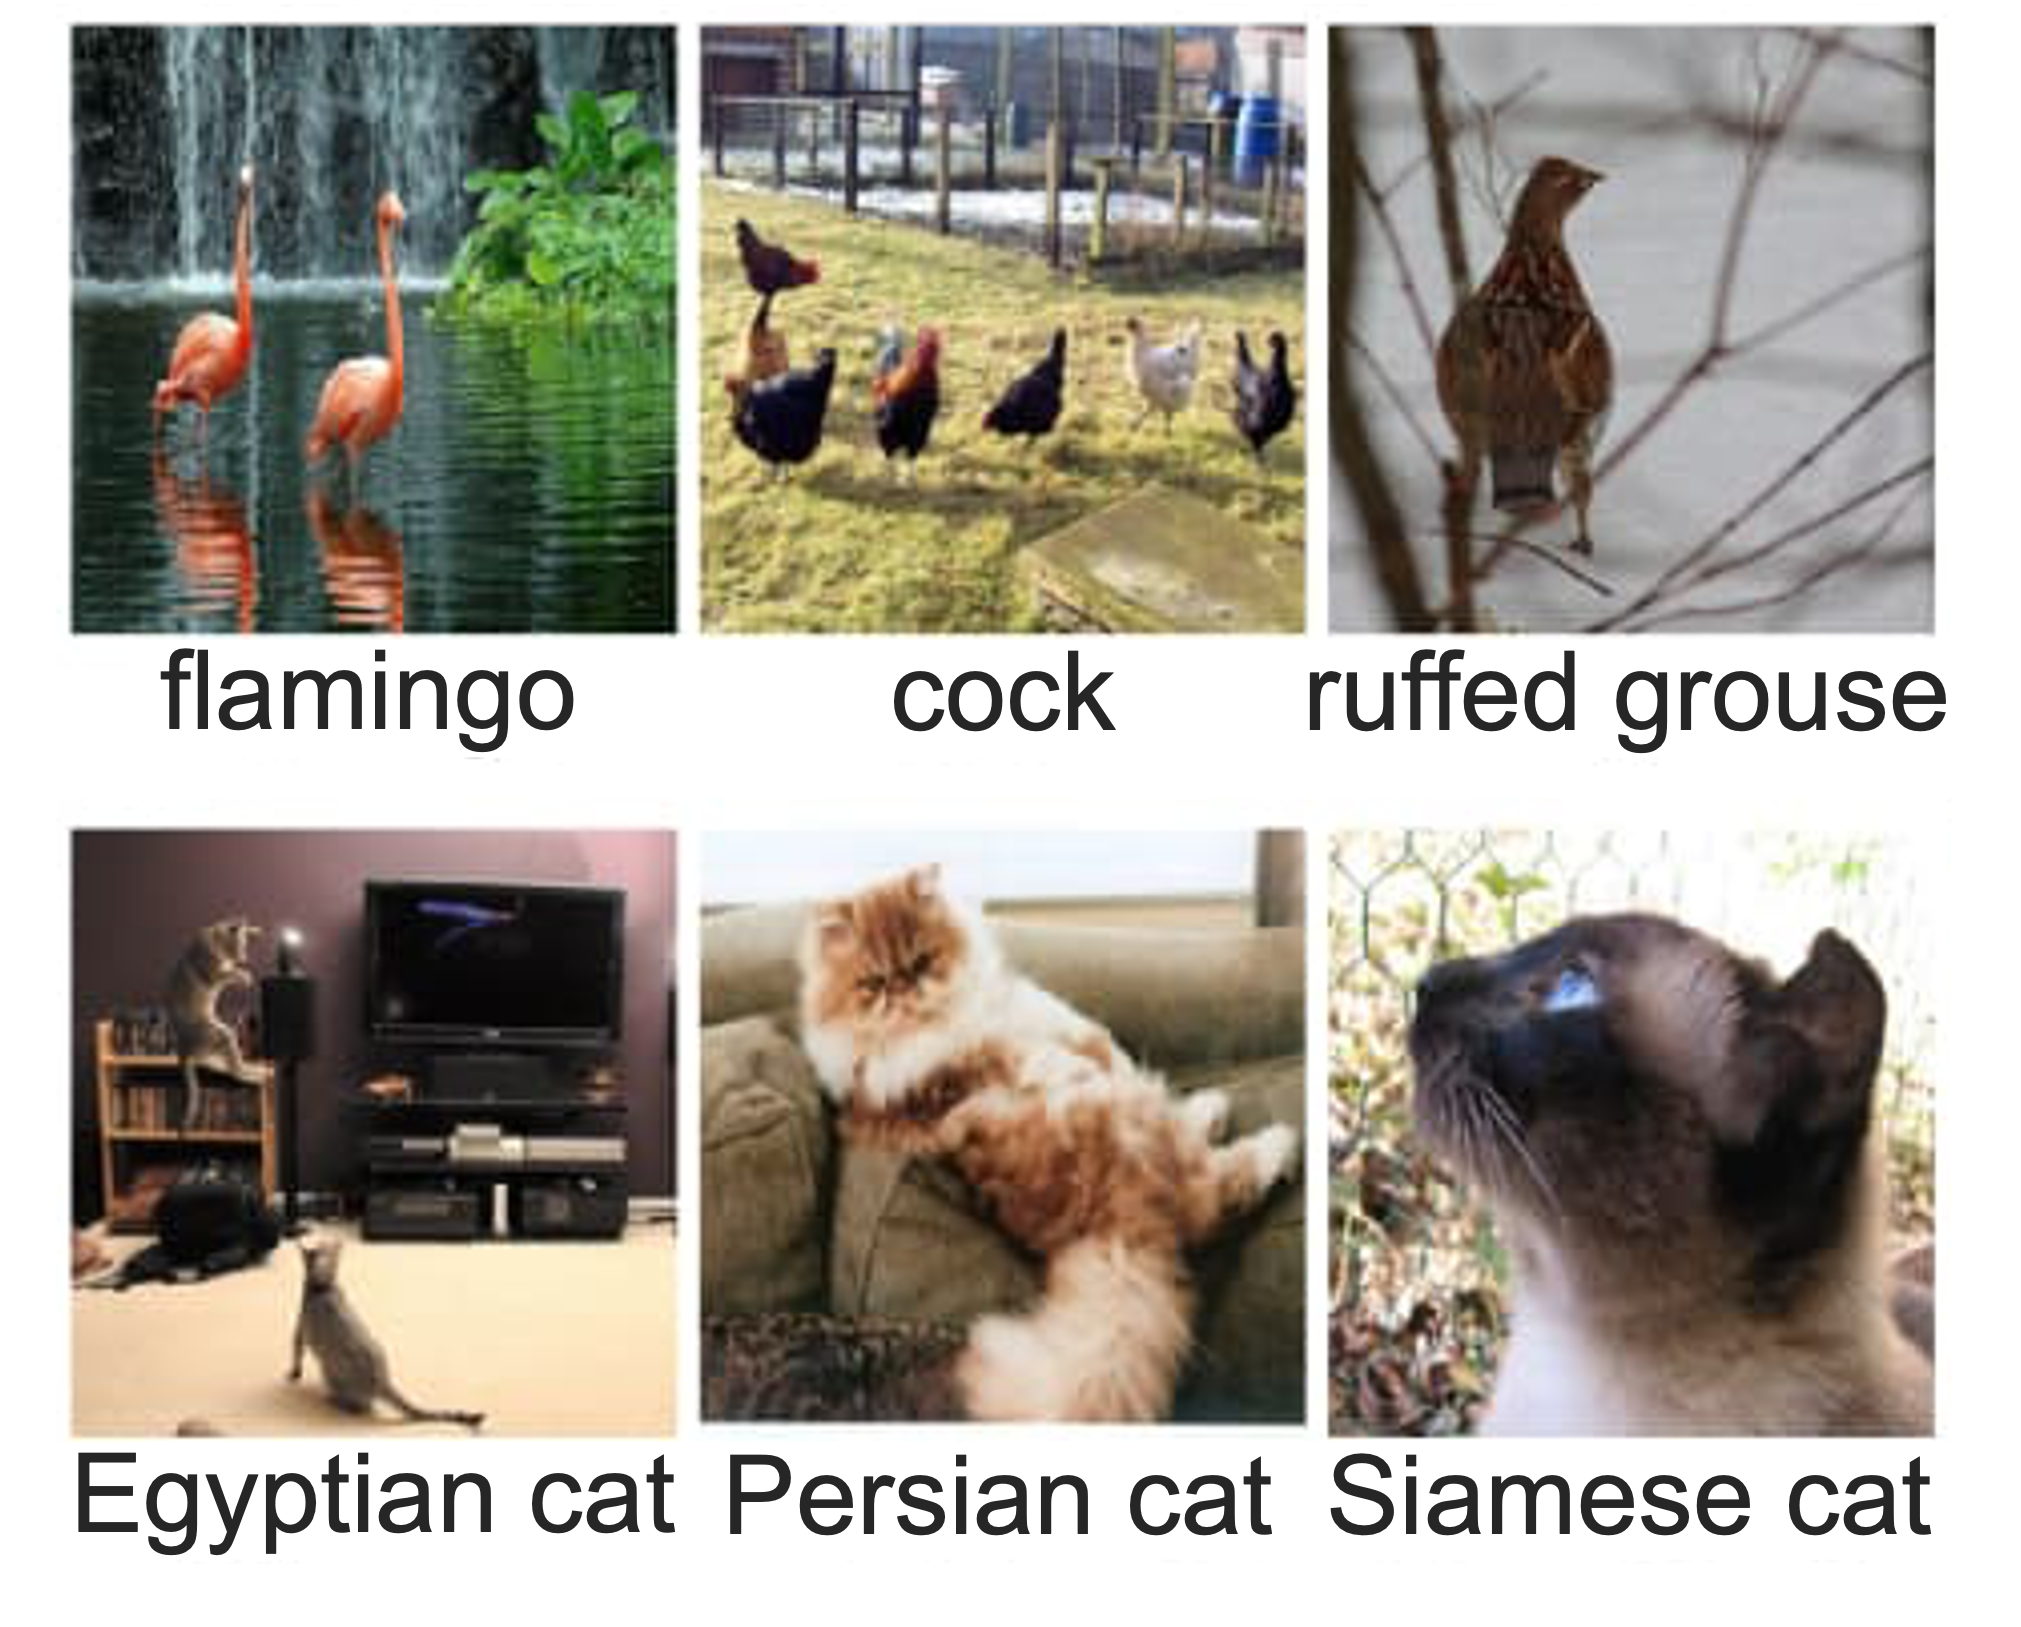
\includegraphics[height=0.9\linewidth, keepaspectratio]{image/imagenet.png}
    \caption{ImageNetの画像例}
    \label{fig:imagenet}
  \end{subfigure}
  \hfill
  \begin{subfigure}[b]{0.45\linewidth}
    \centering
    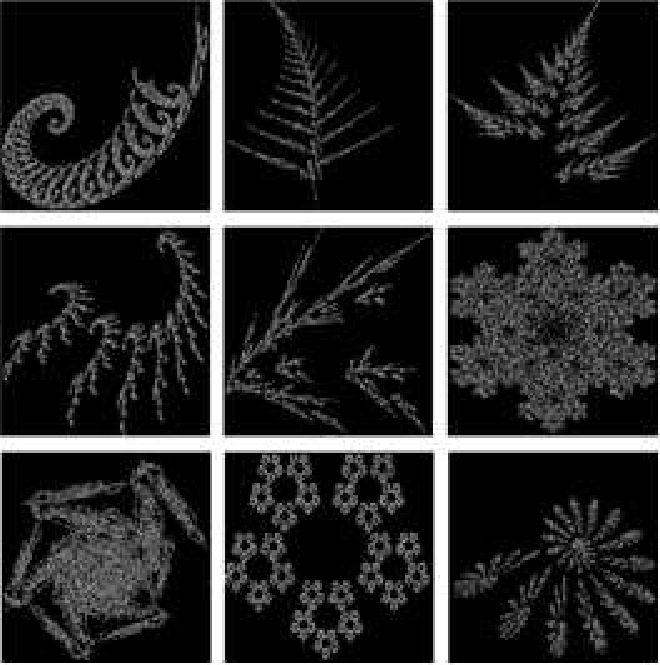
\includegraphics[height=0.9\linewidth, keepaspectratio]{image/fdsl.png}
    \caption{FDSLの画像例}
    \label{fig:fdsl}
  \end{subfigure}
  \caption{ImageNetとFDSLの画像例}
  \label{fig:transfer_learning}
\end{figure}

\subsection{メタ学習}

メタ学習は,学習方法の学習として知られており,FSLにおける効率的なアプローチとして広く認識されている.
図 \ref{fig:meta-learning}にメタ学習の概要図を示す.
% 
\begin{figure}[tbp]
  \centering
  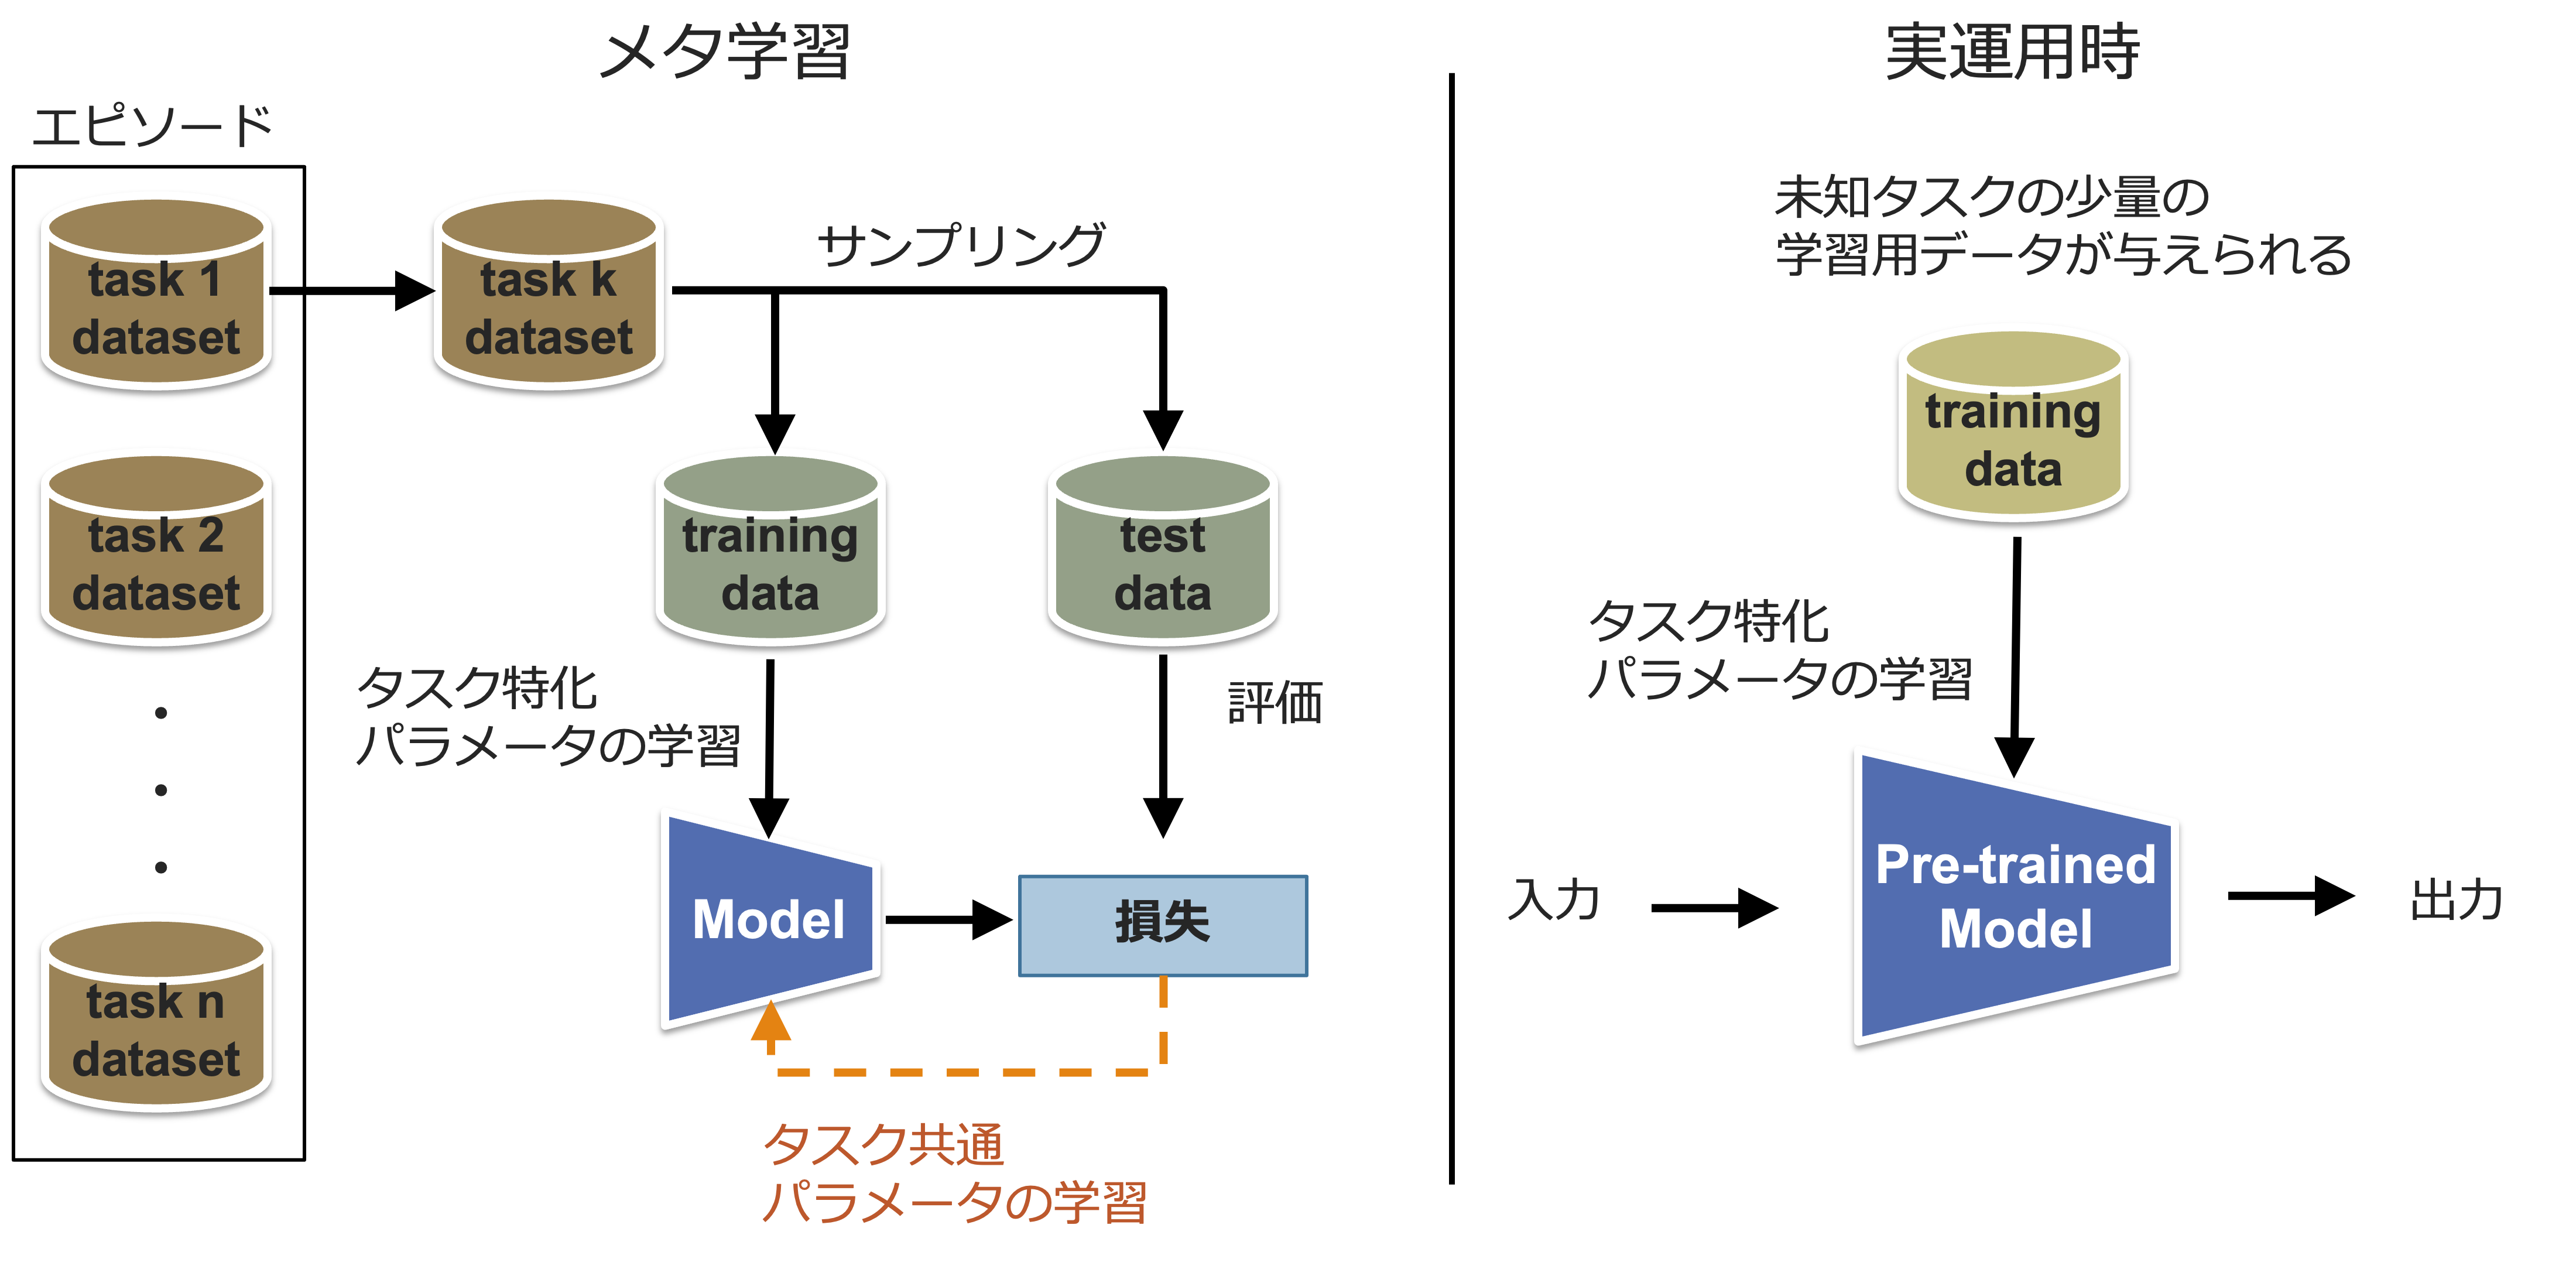
\includegraphics[width=\linewidth, keepaspectratio]{image/meta-learning.png}
  \caption{メタ学習の概要}
  \label{fig:meta-learning}
\end{figure}
% 
メタ学習では,様々なタスクによって構成される学習単位をエピソードと呼び,深層学習モデルは複数のエピソードを通じて学習アルゴリズムを改善し,限られたデータに対する汎化性能を強化する.
各タスクは,それぞれ$K$個のデータを持つ$N$個のクラスで構成されており,このタスク設定は$N$-way, $K$-shot分類と呼ばれる.

メタ学習の各エピソードでは,ランダムに選択された学習タスクに基づいてモデルパラメータが更新される.
このプロセスにより,ネットワークは各エピソードで異なるタスクへの対応を求められるため,特定のサブセットではなく,より一般的な特徴表現の獲得が期待される.

Snellらは,FSLの代表的なメタ学習手法であるPrototypical Networks (ProtoNet) を提案した \cite{protonet}.
ProtoNetの概要を図 \ref{fig:protonet}に示す.
% 
\begin{figure}[tbp]
  \centering
  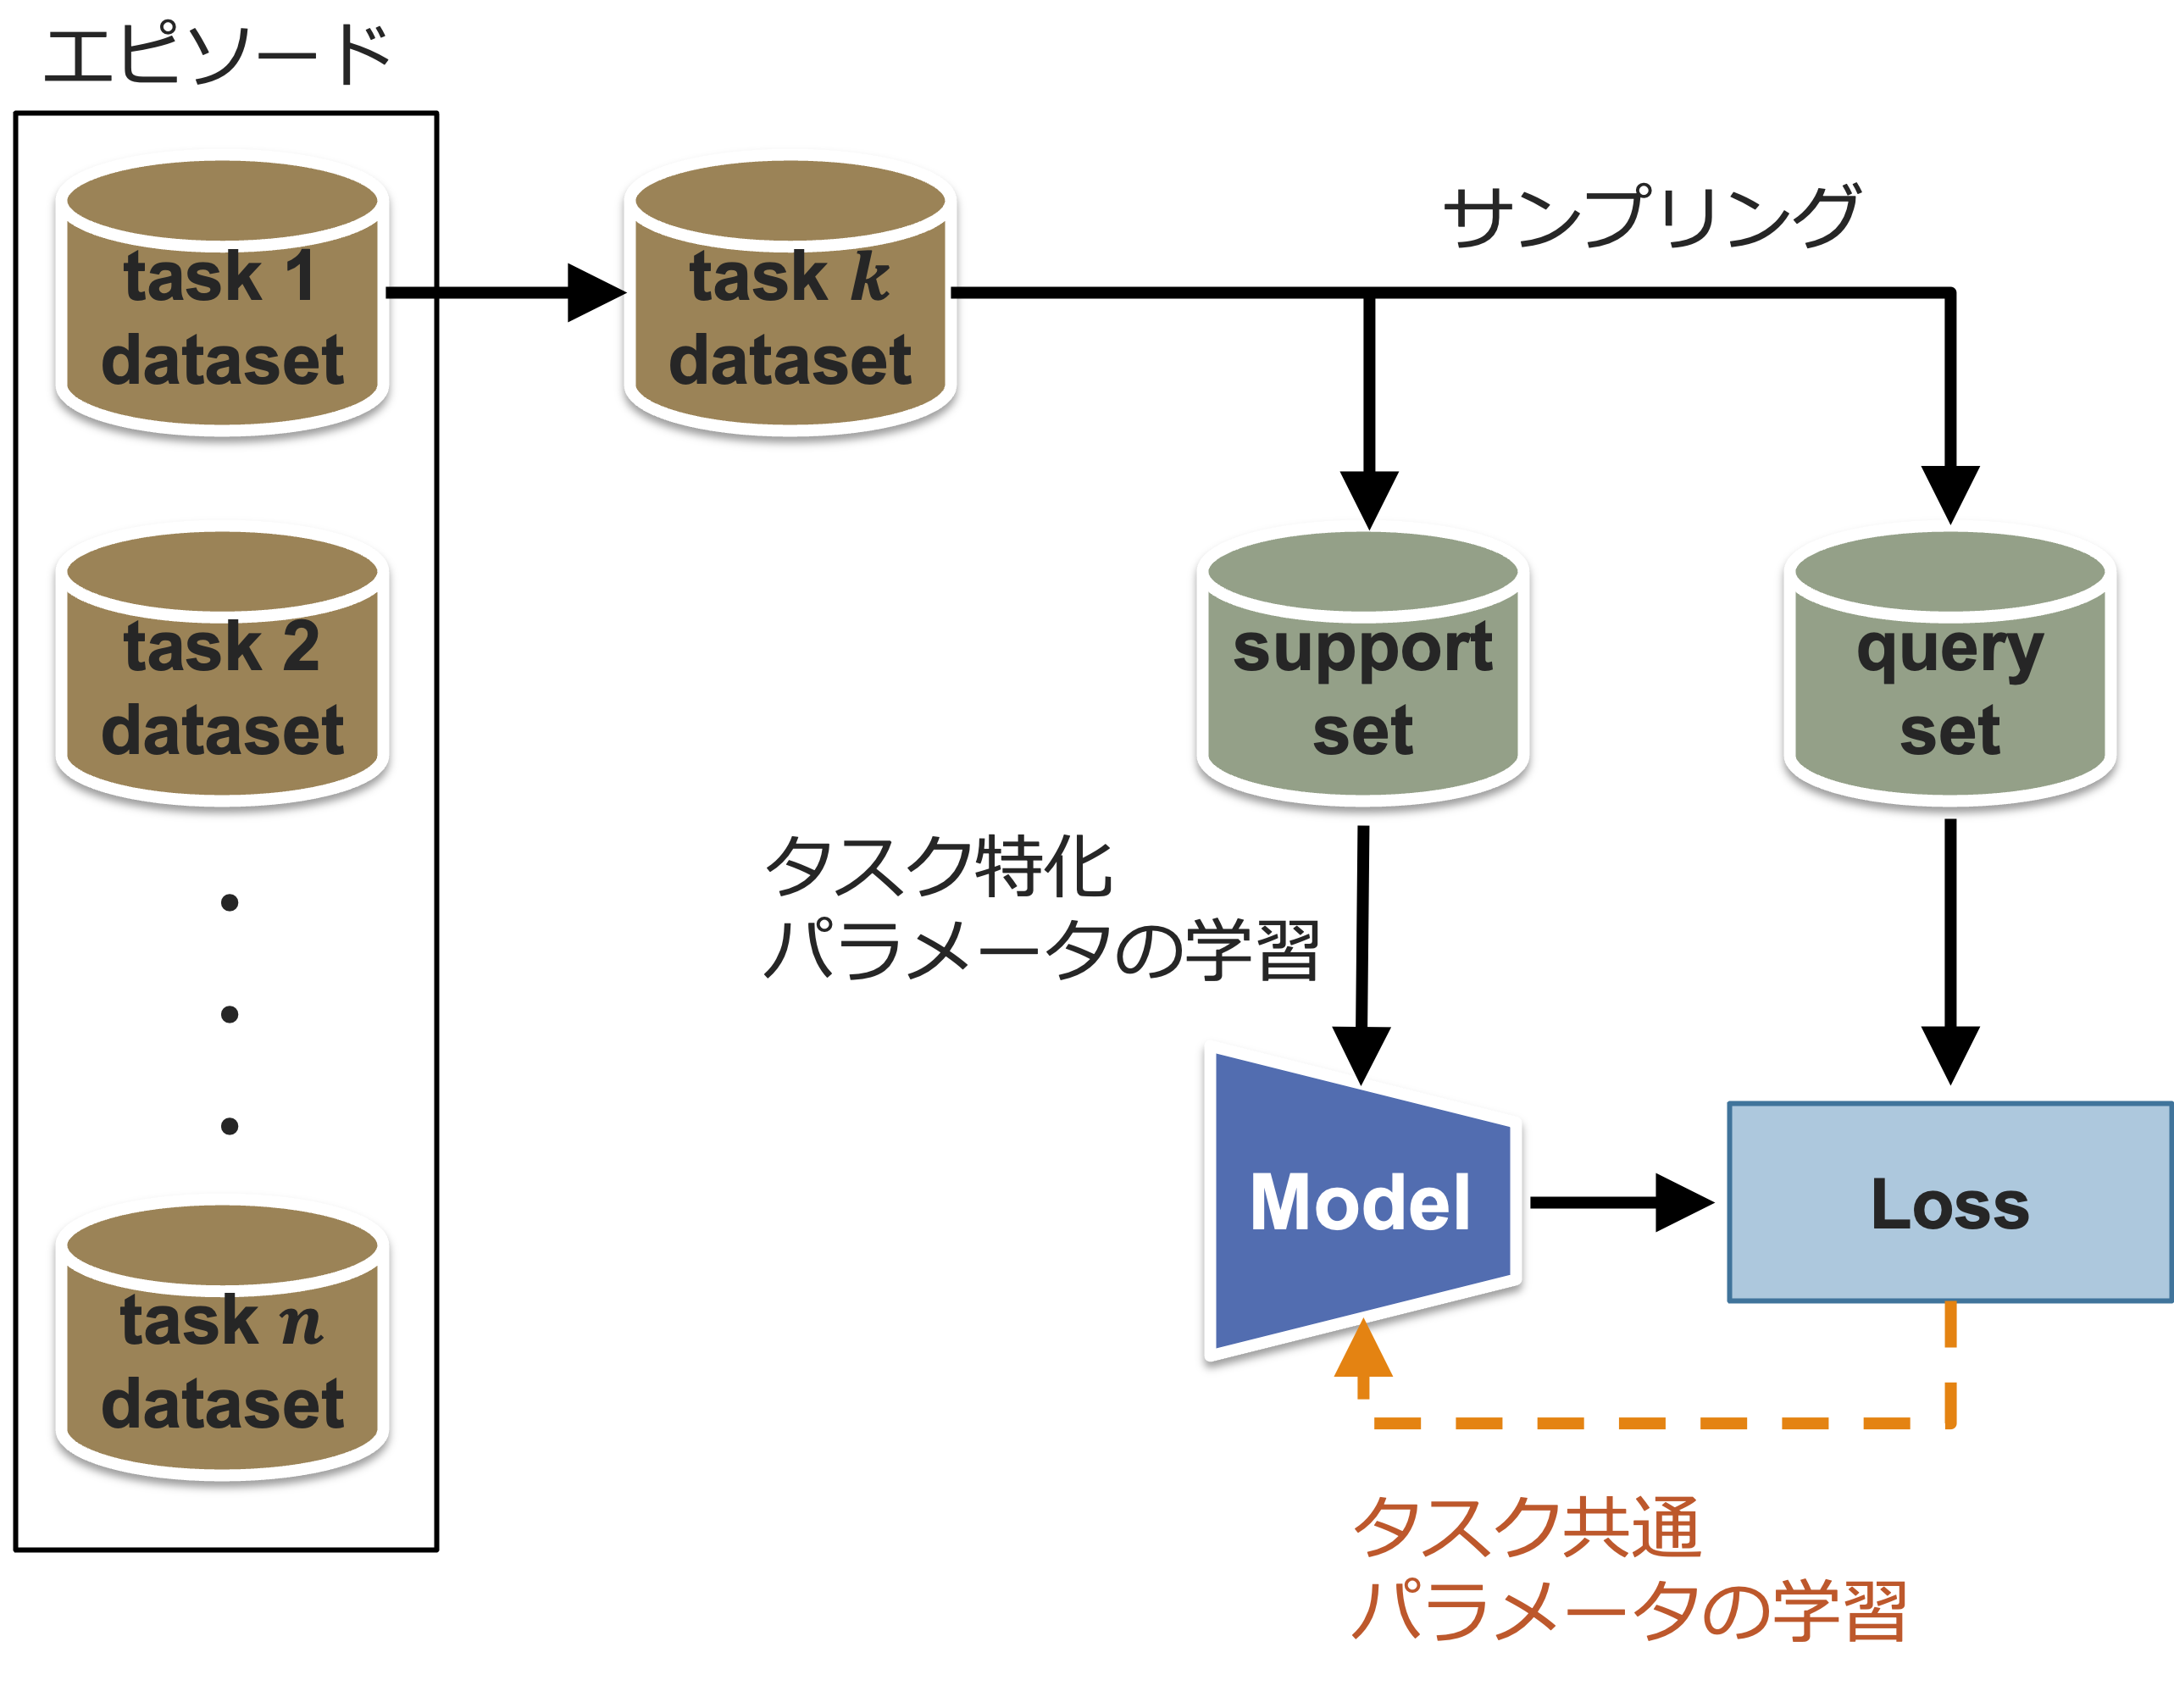
\includegraphics[width=0.7\linewidth, keepaspectratio]{image/protonet.png}
  \caption{ProtoNetの概要}
  \label{fig:protonet}
\end{figure}
% 
ProtoNetでは,モデルに登録するクラスセットであるサポートセット (support-set) と,サポートセットを評価するためのクエリセット (query-set) を用いて学習を行う.
ProtoNetは,入力データと各クラスのプロトタイプとの距離に基づき分類のための特徴空間を学習することにより,少数データにおける分類を実現する.
プロトタイプはサポートセットの埋め込みベクトルの平均として定義される.
具体的に,サポートデータは各クラスのプロトタイプを中心としたクラスタを形成するような空間に埋め込まれ,分類時には,クエリデータの埋め込みベクトルに最も近いプロトタイプを持つクラスが予測クラスとして分類される.
このような距離に基づく分類手法により,FSLにおいて課題となる過学習に対処している.

近年,メタ学習アルゴリズムがFew-Shot Open-Set Recognition(FSOSR) の分野に拡張され,登録クラスの分類と未登録クラスの検出の両方を同時に高い精度で実現する手法が提案された.
Liuらは,学習過程で登録クラスの分類と未登録クラスの検出に取り組むPEELERアルゴリズムを提案した \cite{peeler}.
従来のソフトマックス分類器は,学習クラスを過剰に適合させる傾向があるため,未登録クラスの検出が困難であった.
PEELERはこの課題に対し,エピソードごとに新規クラスをランダムに選択し,これらのクラスの事後エントロピーを最大化することにより未登録クラスの検出能力を向上させる.
さらに,メタ学習をオープンセット認識に拡張したことにより,より一般化された特徴抽出における表現力を獲得し,認識タスクの様々なスケールや複雑さに対して効果的な学習フレームワークを提供する.
% さらに,エピソード学習と未登録クラスに対する損失関数を組み合わせることにより,より一般化された特徴抽出における表現力を獲得し,認識タスクの様々なスケールや複雑さに対して効果的な学習フレームワークを提供する.

PELLERの概要を図 \ref{fig:peeler}に示す.
% 
\begin{figure}[tbp]
  \centering
  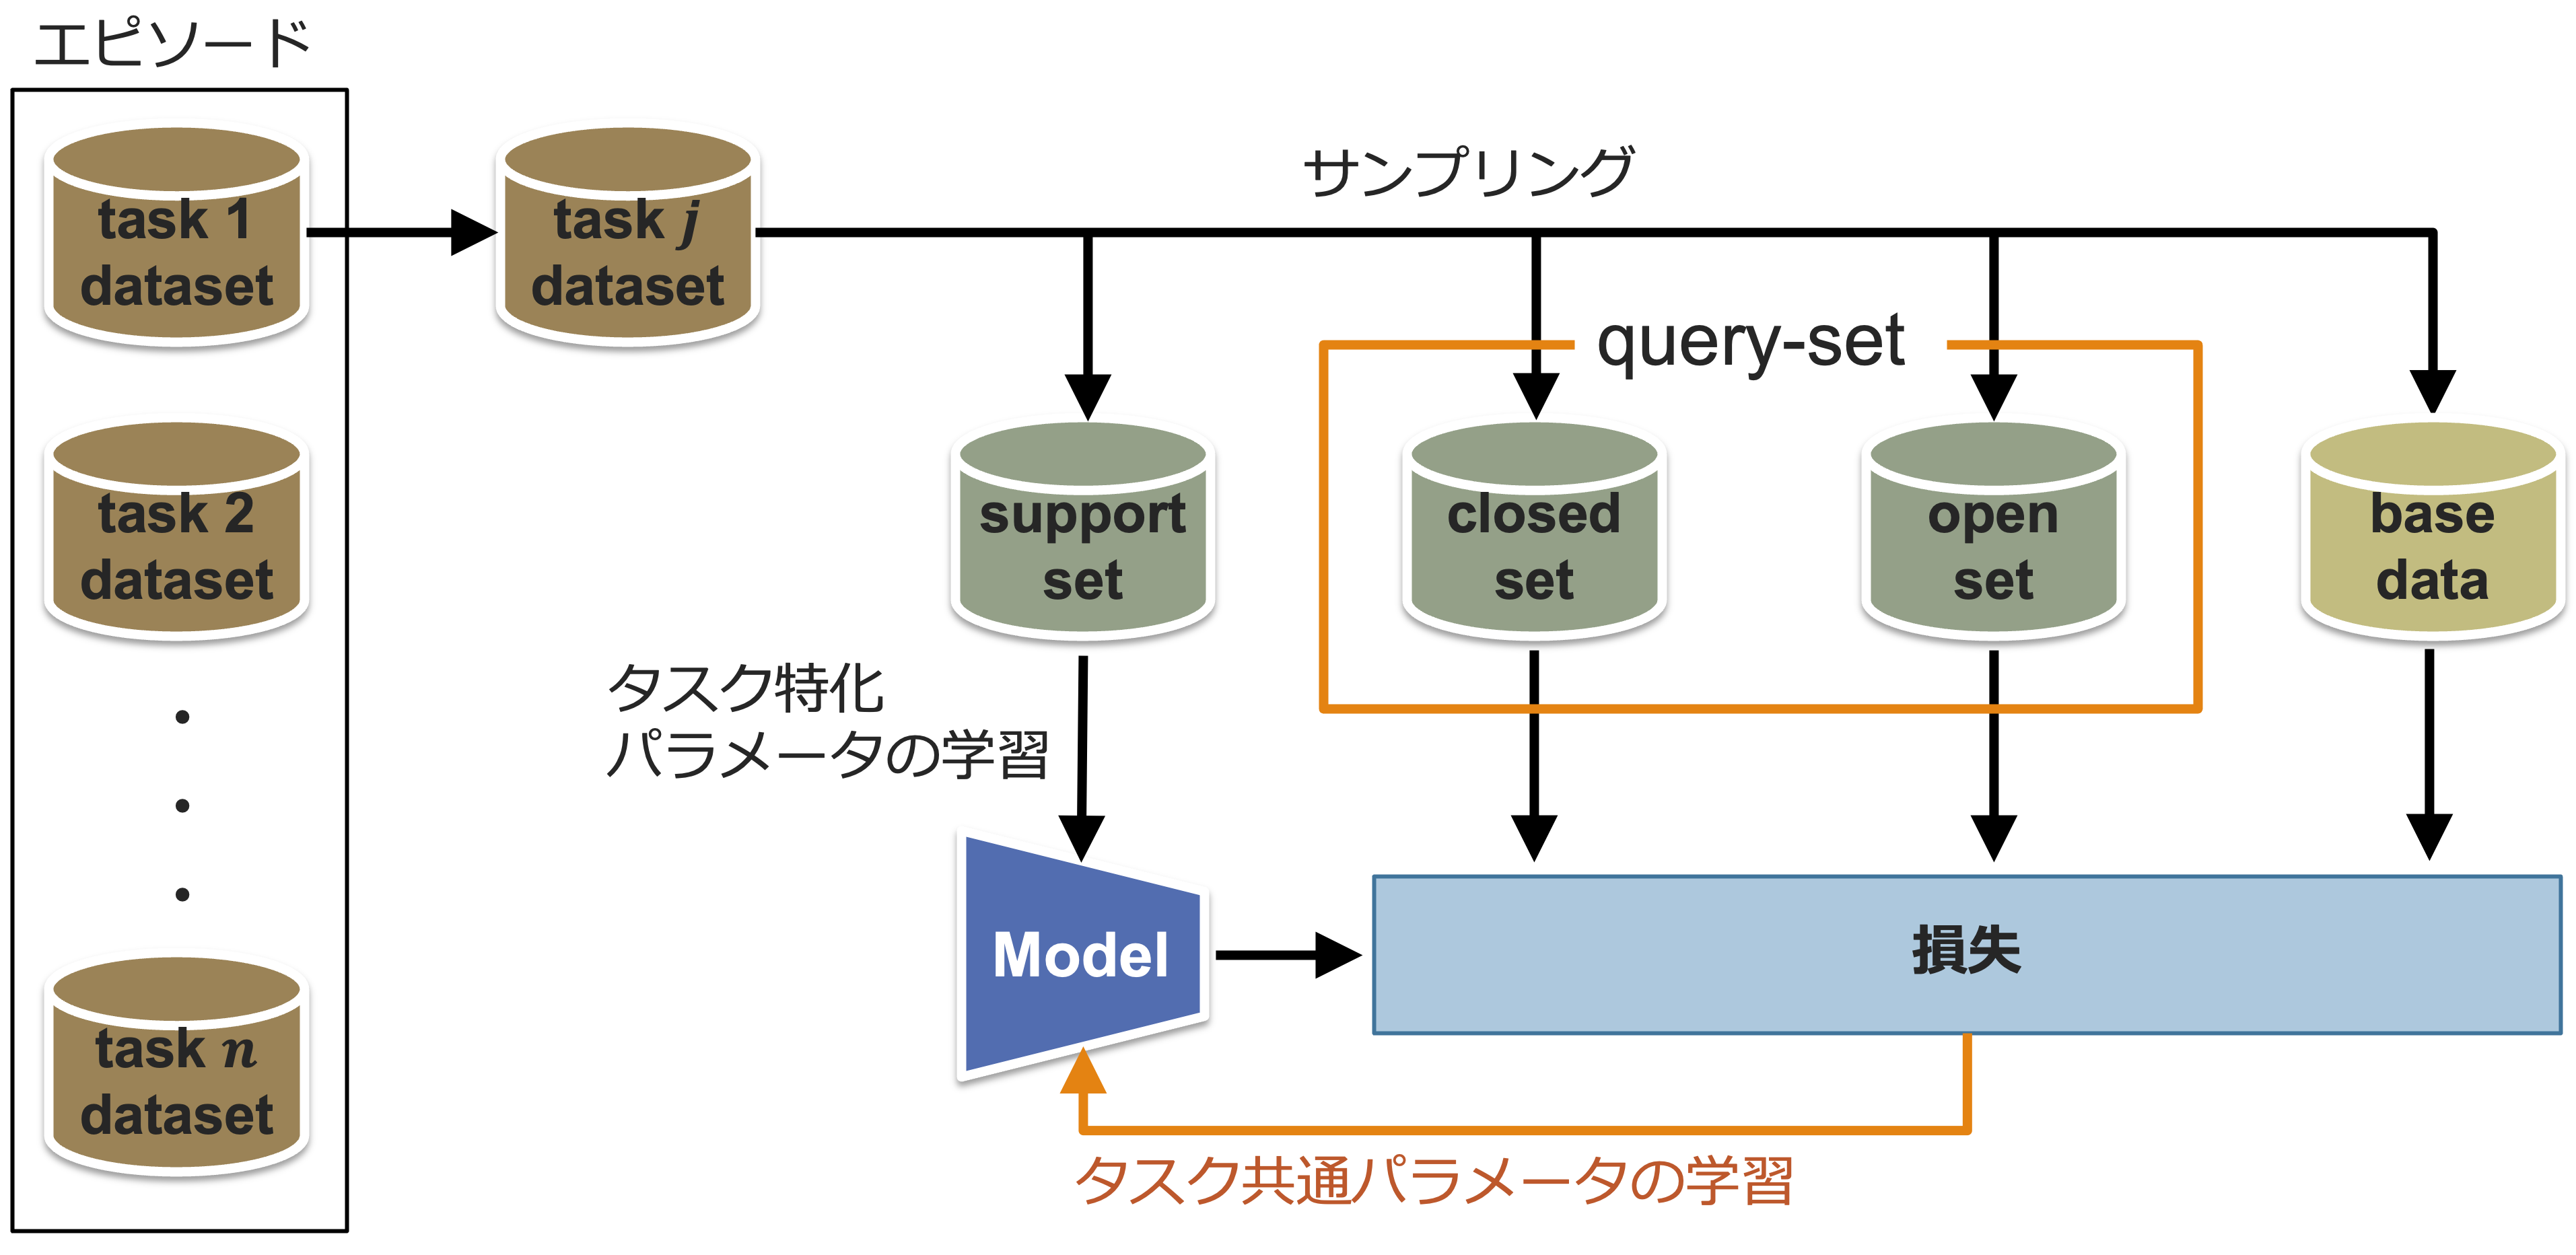
\includegraphics[width=\linewidth, keepaspectratio]{image/peeler.png}
  \caption{PEELERの概要}
  \label{fig:peeler}
\end{figure}
% 
各タスクではサポートセット (support-set) と呼ばれる登録用データとクエリセット (query-set) と呼ばれる評価用データを使用する.
さらにクエリセットはサポートセットと同じクラスから構成されるクローズドクエリセット (closed-query set) と,サポートセットと異なるクラスから構築されるオープンクエリセット (open-query set) の2つに分けられる.
サポートデータ,クローズドクエリデータ,オープンクエリデータの選択方法の概要を図 \ref{fig:peeler_data}に示している.
% 
\begin{figure}[tbp]
  \centering
  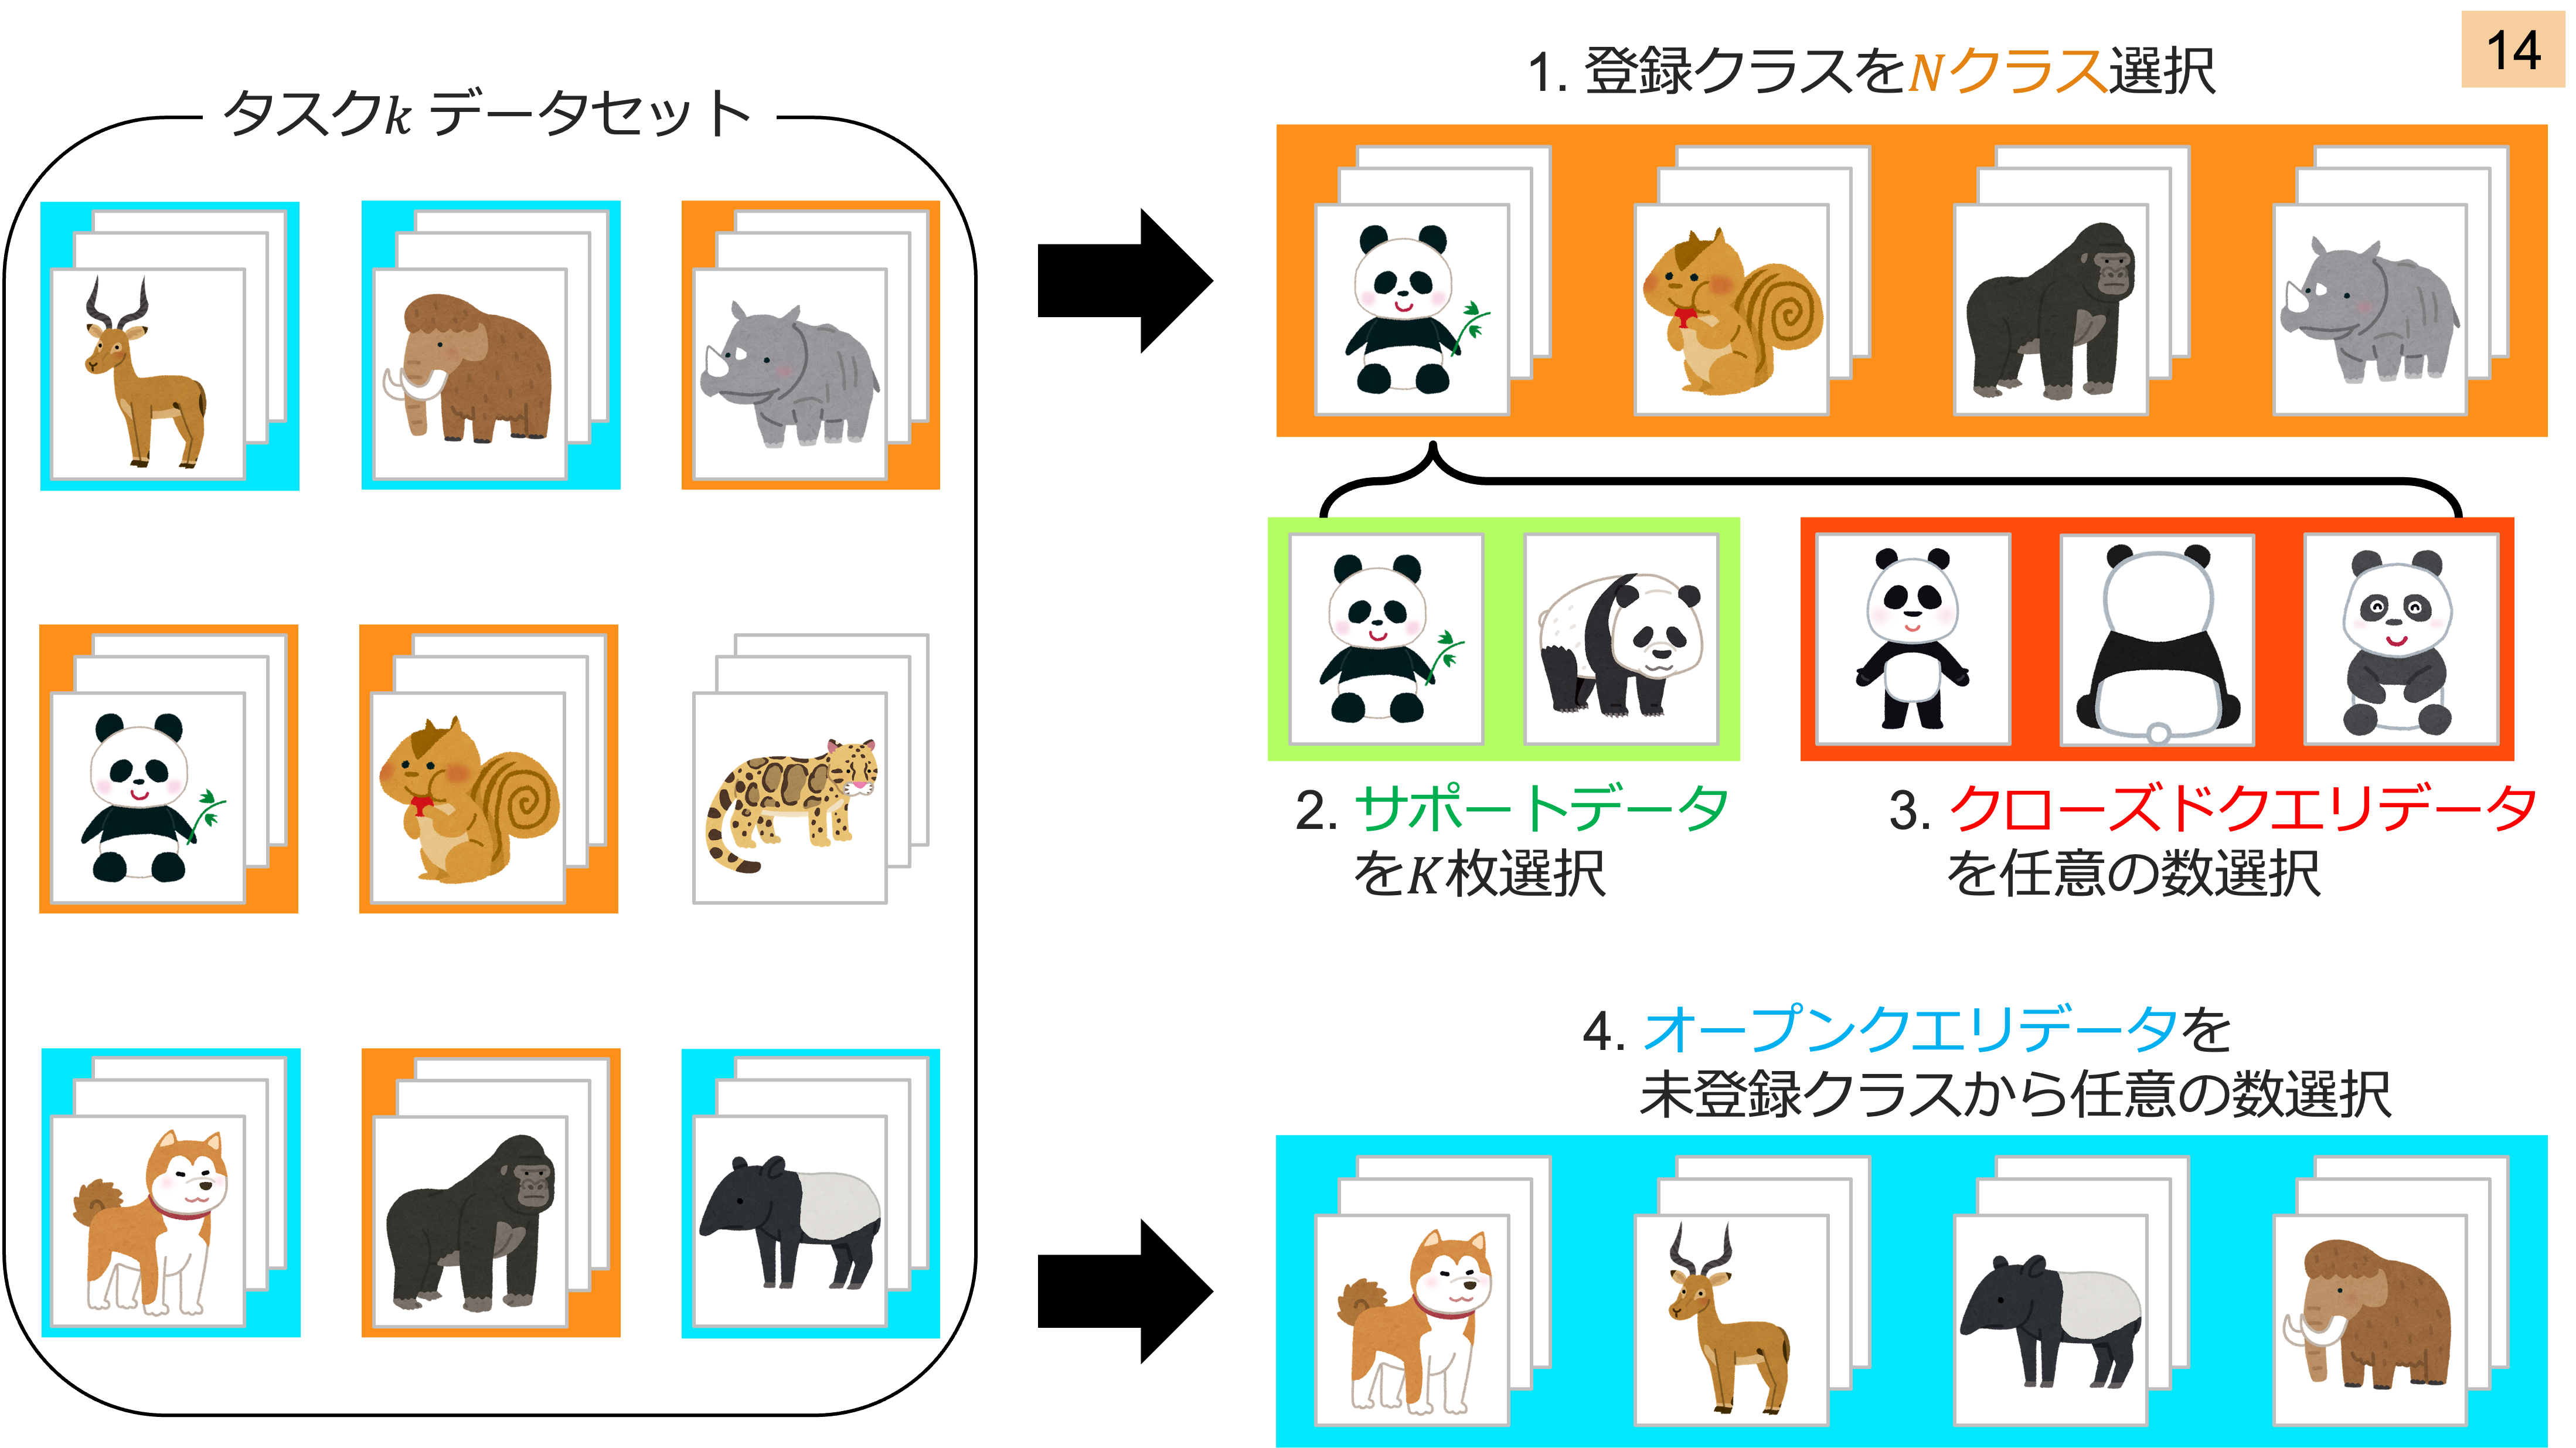
\includegraphics[width=\linewidth, keepaspectratio]{image/meta-class.png}
  \caption{登録クラス・未登録クラスの選択方法}
  \label{fig:peeler_data}
\end{figure}
%
PEELERは,プロトタイプと入力データとの距離に基づいて分類を行う.
具体的には,クエリデータが各プロトタイプの閾値より大きい場合は未登録クラス,閾値よりも小さい場合は最も近いプロトタイプのクラスに分類される.
PEELERはモデルに登録されたクラスの分類と未登録クラスの検出において高い精度を達成するため,FSL損失,OSR損失,分類損失の3つの異なる損失関数を採用している.
FSL損失は,プロトタイプとクローズドクエリセットを近づけることで,少数データにおける登録クラスの分類性能を向上させる.
OSR損失はプロトタイプとオープンクエリセットを離すことで,未登録クラスの検出精度を向上させる.
最後に,分類損失は,ランダムな画像から構成されるベースデータから適切な特徴を抽出し,モデルの分類能力を最適化するように設計されている.
エピソードを通してタスク間で異なるクラスセットを学習することにより,モデルは特定のタスクではなく,タスク間の共通性を学習することが期待される.

FSL損失の導出には,学習用データセットから選択されるサポートデータとクローズドクエリデータが用いられる.
% $N$-way, $K$-shot分類において,サポートデータは,学習用データセットから$N$クラス$K$枚ずつランダムに選択される.
% 一方,クエリデータは,サポートセットを用いた分類能力を評価するためのクラスデータであり,サポートセットと同じモデルに登録するクラスセットから選択される.
% 一方,クエリデータは,テストの際に分類精度を確かめるために使用されるテストデータを模したデータであり,学習用データセットのサポートセットと同じクラスに属する別の画像からランダムに選択される.
メタ学習の過程において,クローズドクエリデータから抽出された特徴ベクトルをサポートデータの正解クラスに近づける学習を行うことで,モデルは正確な分類を実現する特徴マッピングが習得可能となる.
図\ref{fig:fsl_loss}では,FSL損失で学習することにより効果的に登録クラスの分類が可能になる例を示している.
以下に具体的なFSL損失の導出過程を述べる.
まず,サポートデータの平均特徴ベクトルであるプロトタイプとクローズドクエリデータの特徴ベクトル間のユークリッド距離を計算する.

\begin{figure}[tbp]
  \centering
  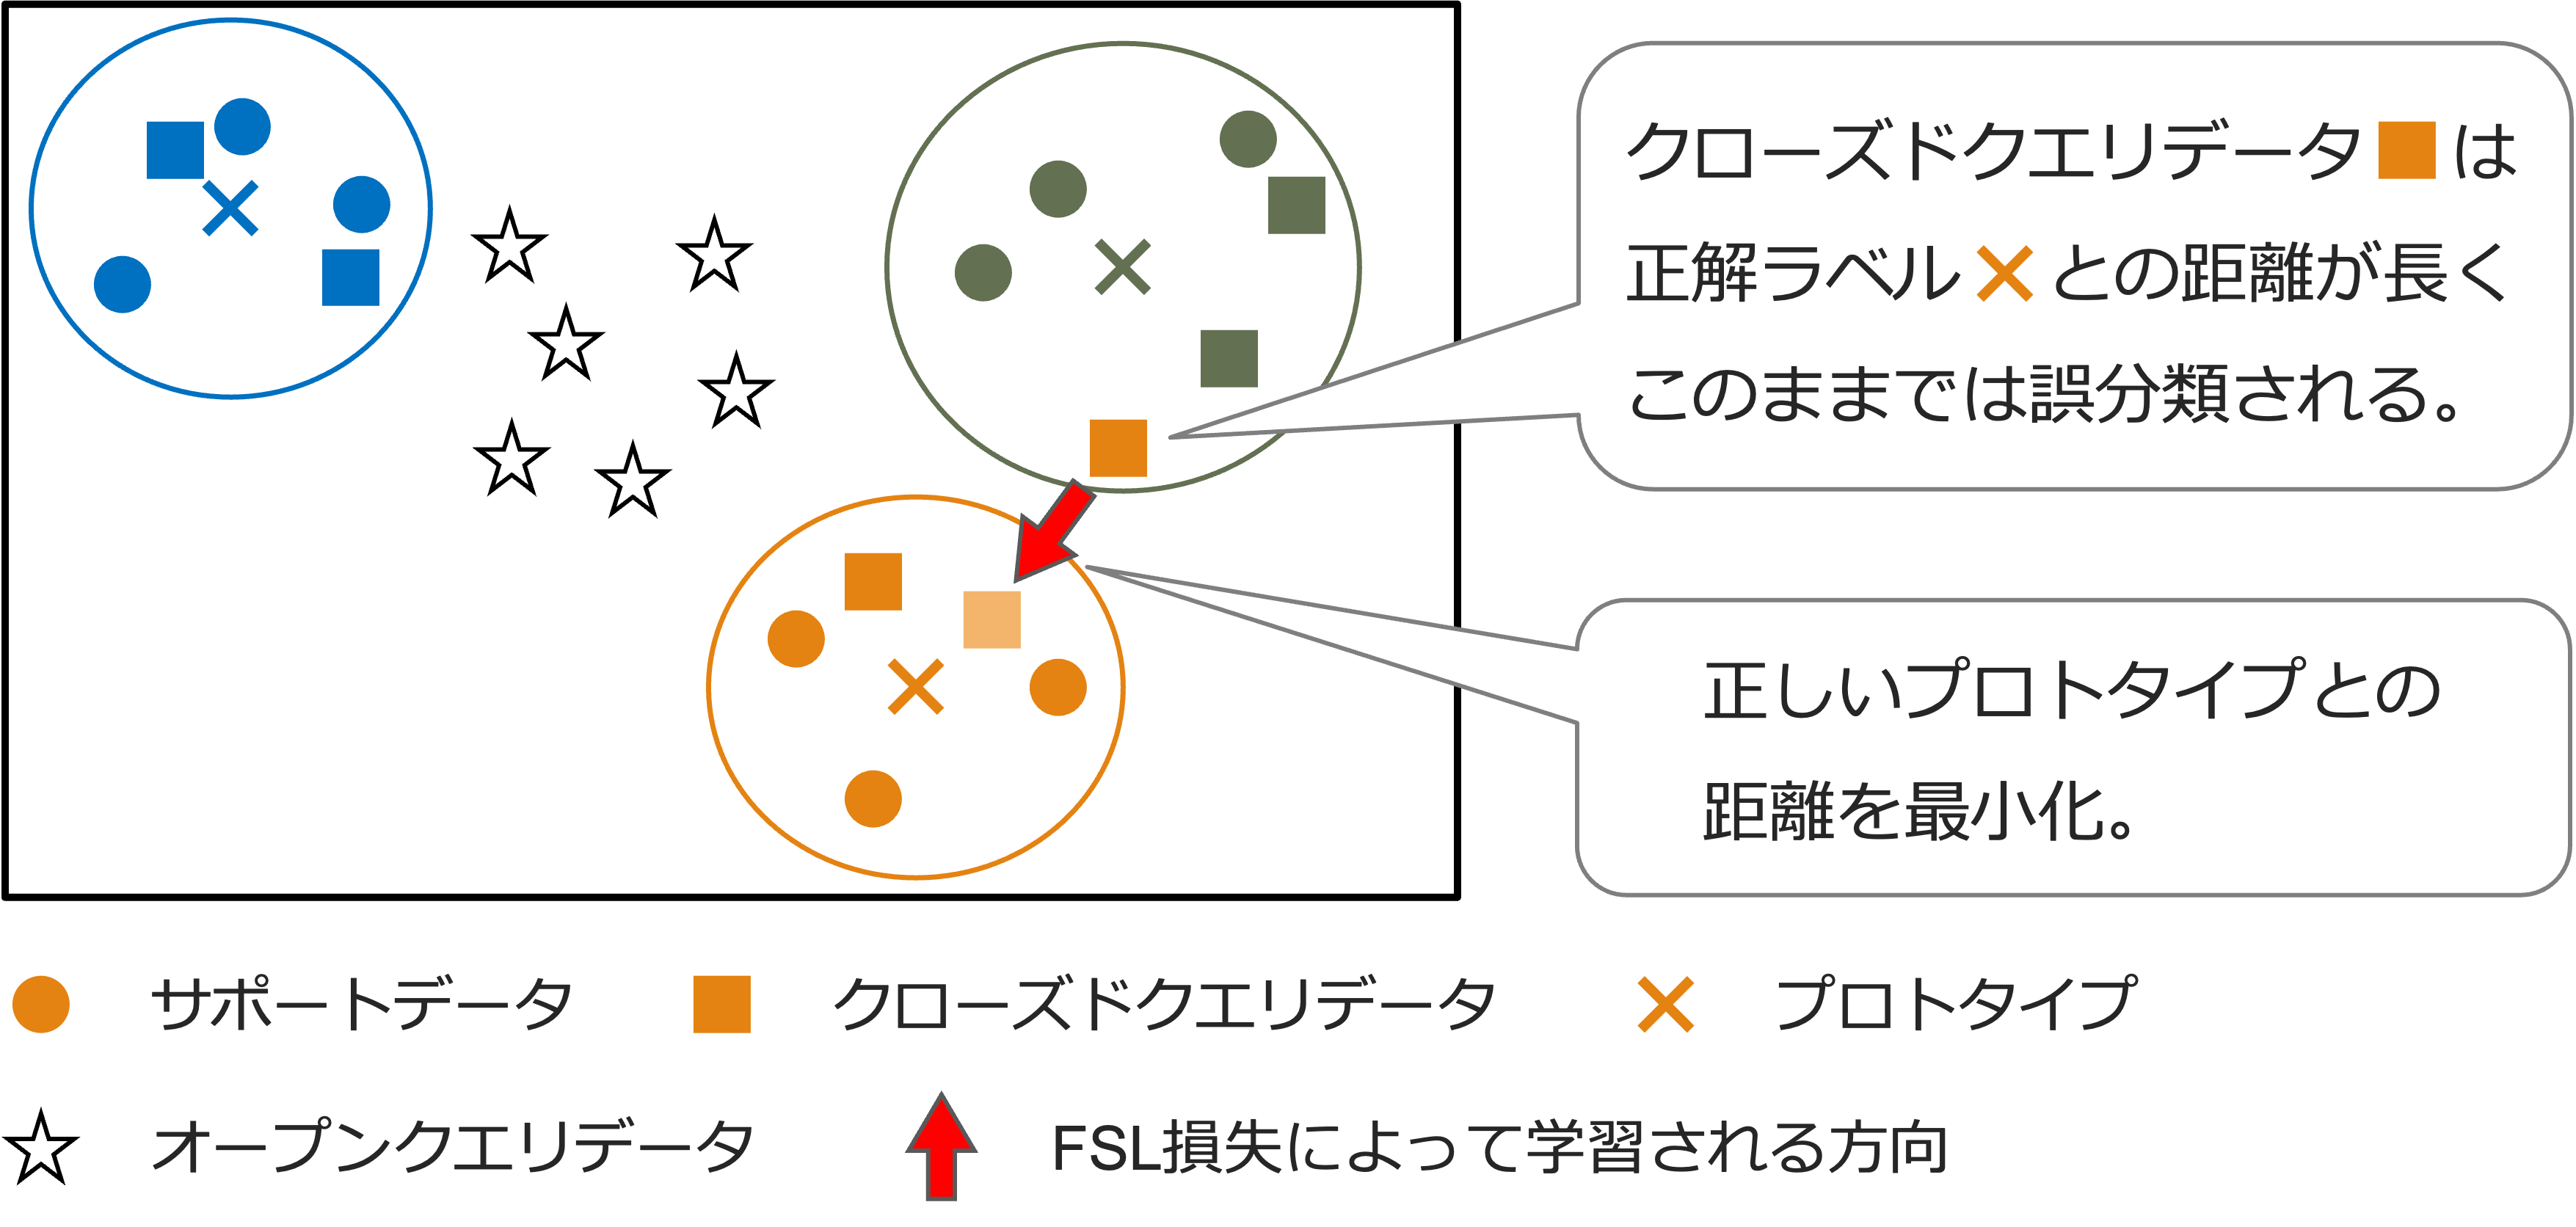
\includegraphics[width=\linewidth, keepaspectratio]{image/fsl_loss.png}
  \caption{FSL損失での学習が登録クラスの分類精度を向上させる例}
  \label{fig:fsl_loss}
\end{figure}

\begin{align}
  d(f_\phi(\mathbf{x}),\mu_{k})=(f_\phi(\mathbf{x}),\mu_{k})^T(f_\phi(\mathbf{x}),\mu_{k})
\end{align}

\noindent
ここで,${f_\phi(\mathbf{x})\in{\mathcal{F}}}$ ,は画像 ${{\mathbf{x}}\in{\mathcal{X}}}$ におけるクローズドクエリデータの特徴ベクトル,$\mu_{k}$ はサポートデータにおける特徴ベクトルの平均を表す.
サポートデータの平均特徴ベクトルであるプロトタイプは以下の式で算出される.

\begin{align}
  \mu_{k}=\frac{1}{|\mathcal{P}_{i,k}|}\sum_{\mathbf{x}_j\in\mathcal{P}_{i,k}}f_\phi(\mathbf{x}_j)
\end{align}

\noindent
ここで,$\mathcal{P}_{i,k}=(\mathbf{x}_j\in\mathbb{S}_i|y_j=k)$は,クラス $k$ におけるサポートデータ集合であり,$\mathbb{S}$ は $i$ 番目の学習の際に選択されたサポートデータ集合である.

次に,ユークリッド距離に負の符号を付けてソフトマックス関数に適用する.

\begin{align}
  p_\phi(y=k|\mathbf{x})=\frac{exp(-d(f_\phi(\mathbf{x}),\mu_{k})}{\sum_{k'}exp(-d(f_\phi(\mathbf{x}),\mu_{k'}))}
\end{align}

サポートデータとクローズドクエリデータの特徴ベクトル間のユークリッド距離が短いほど,正しく分類できる確率が高くなる.
よって,この距離が長い場合に大きな損失を与えることが望ましい.
最終的に,FSL損失はクロスエントロピー損失を用いて計算される.
一般的なクロスエントロピー損失は以下の通り定義される.

\begin{align}
  \mathcal{L}_{CE}=\sum_{(x_i,y_i)}-\textrm{log}\,p(y_i,\mathbf{x}_i)
\end{align}

OSR損失の計算の際は,学習用データセットから選択されるサポートデータとオープンクエリデータが用いられる.
ここでのサポートデータは,前述したFSL損失の計算時に利用したものと同一である.
一方,オープンクエリデータは,未登録クラスの検出能力を確かめるための入力データであり,学習用データセットからサポートセットと異なるクラスの画像がランダムに選択される.

メタ学習の過程において,オープンクエリデータから抽出された特徴ベクトルをプロトタイプから遠ざけることにより,深層学習モデルは正確な未登録の検出能力を習得することが期待される.
図 \ref{fig:osr_loss}に,OSR損失で学習することにより効果的に未登録クラスの検出が可能になる例を示す.

\begin{figure}[tbp]
  \centering
  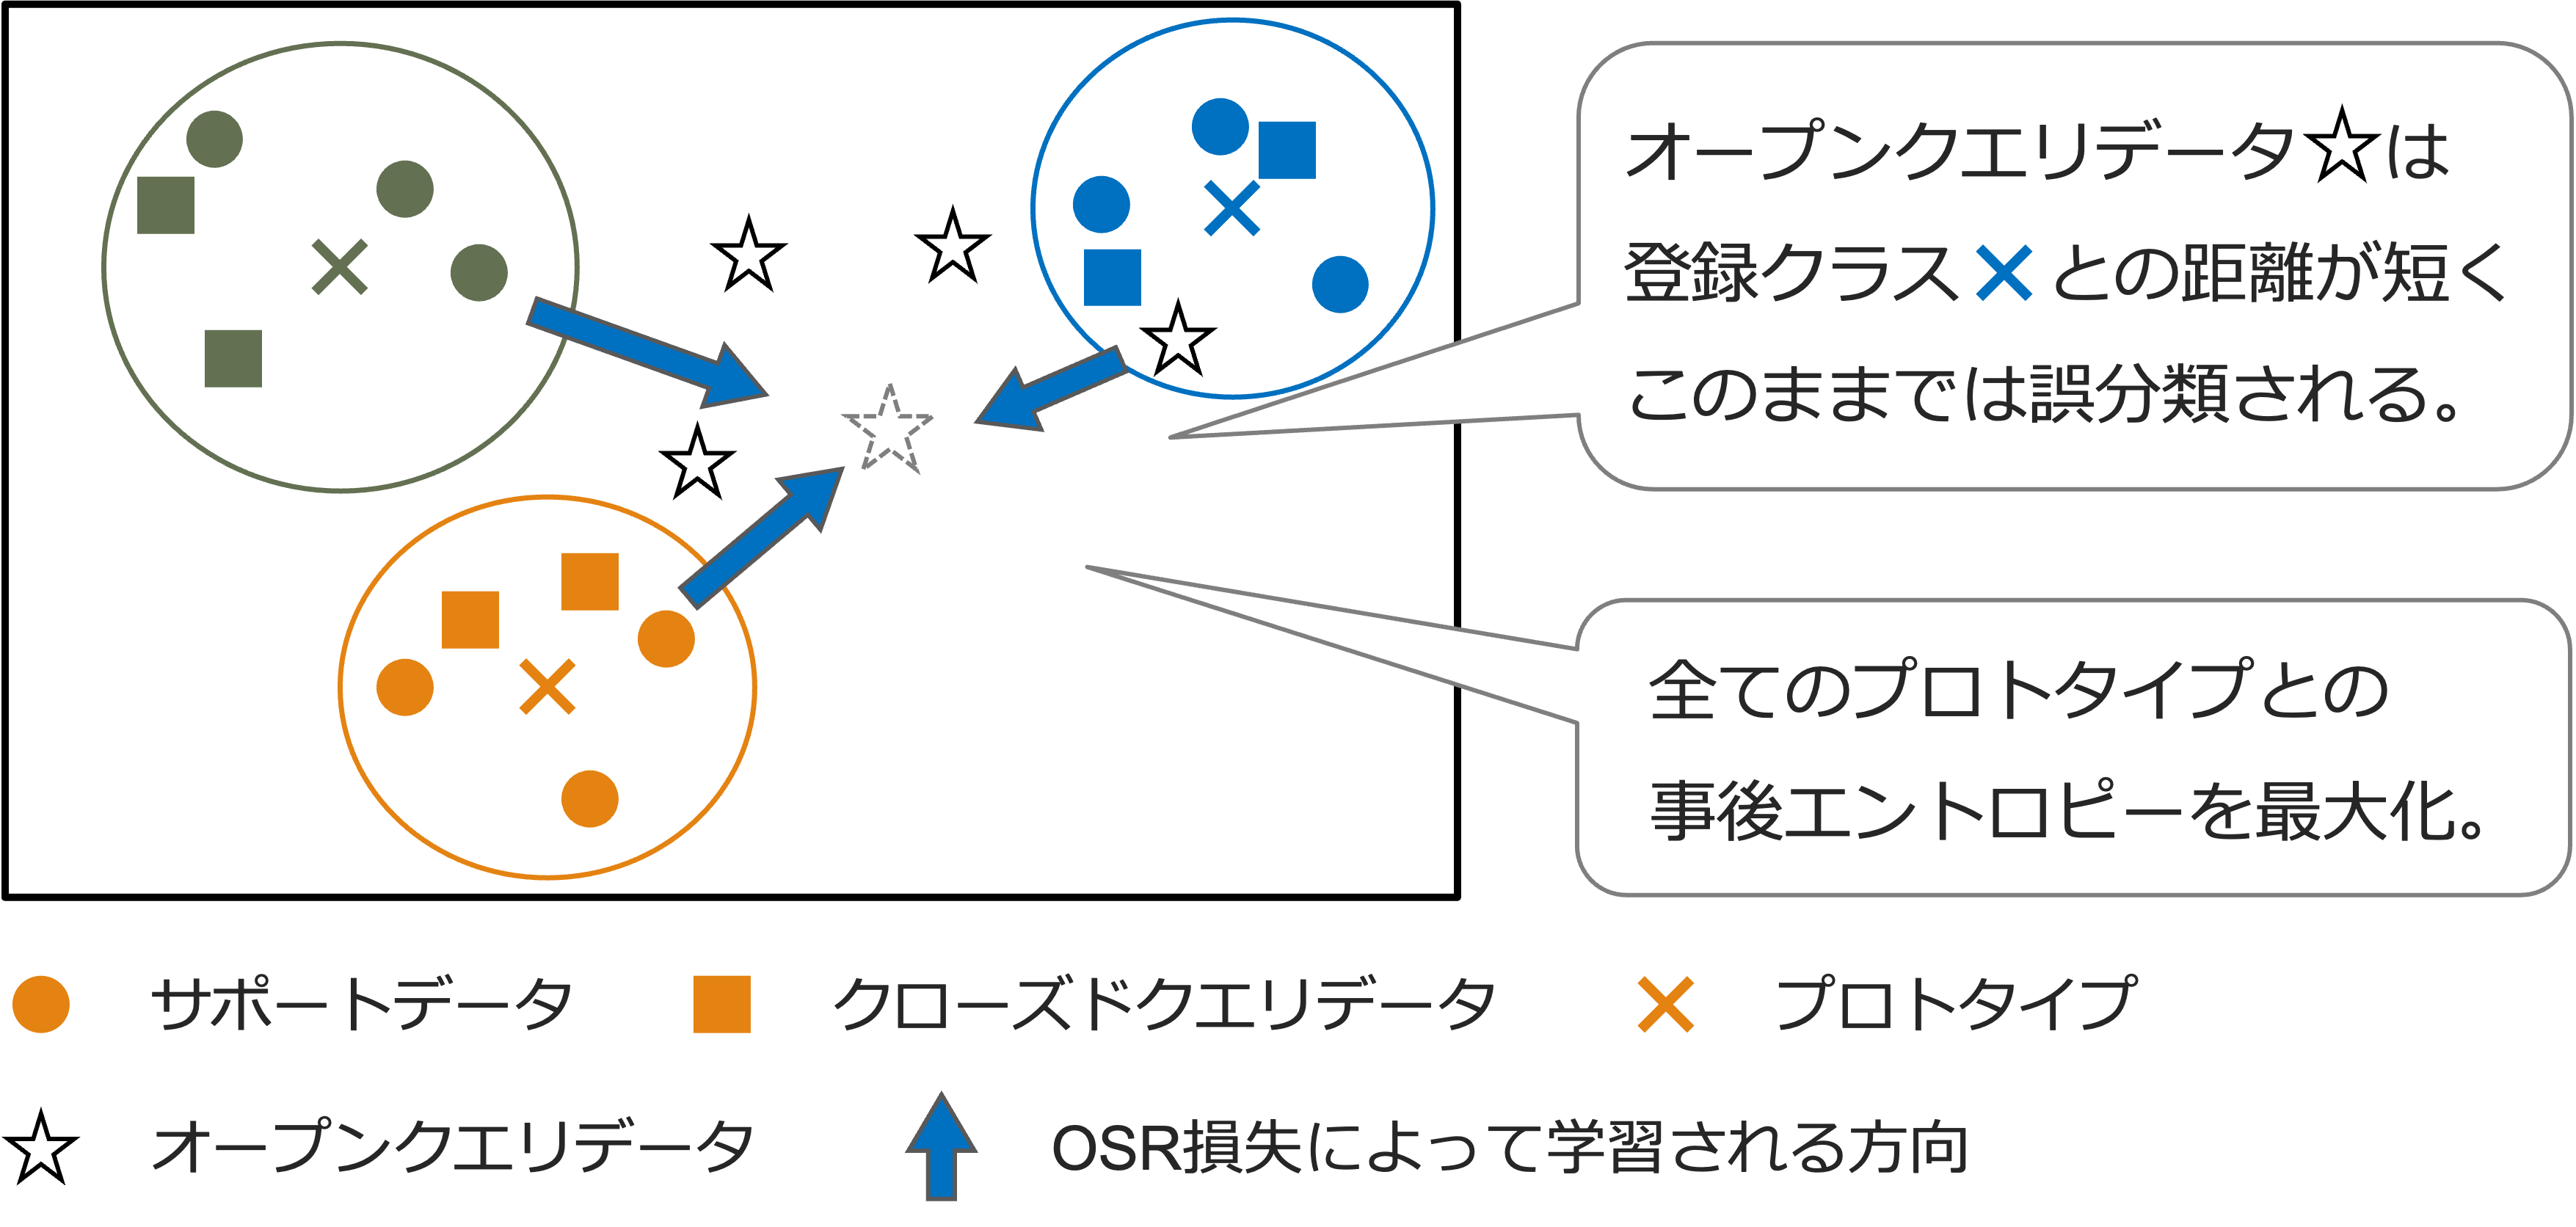
\includegraphics[width=\linewidth, keepaspectratio]{image/osr_loss.png}
  \caption{OSR損失での学習が未登録クラスの検出精度を向上させる例}
  \label{fig:osr_loss}
\end{figure}

以下に具体的なOSR損失の導出過程を述べる.
モデルは,正しく未登録の検出を行うために,未登録クラスからのサンプルに遭遇した際,サポートデータのどのクラスにおいても大きな確率を割り当てるべきではない.
この場合,サポートデータにおける最大のクラス確率$ \mathrm{max_k}\,p_\phi(y=k|\mathbf{x}) $が小さければ,未登録クラスのサンプルを適切に棄却することができる.
この目的を達成するため,学習アルゴリズムは,オープンクエリデータのサンプルに対して,サポートデータのクラス分類確率の最小化を図る.
これは,オープンクエリデータの事後エントロピーを最大化すること,すなわち負のエントロピーを用いることで実現可能である.

\begin{align}
    \mathcal{L}_{osr}[\mathbf{x}]=\sum_{k\in\mathbb{C}_i}p(y=k|\mathbf{x})\,\textrm{log}\,p(y=k|\mathbf{x})
\end{align}

\noindent
ここで,$\mathbb{C}_i$はオープンクエリデータのクラス集合である.

分類損失の導出では,タスク$k$データセットから任意の数の画像枚数がベースデータとして選択される.
この分類損失は,モデルが新しいドメインにおける分類タスクに対して,一般的かつ有用な特徴抽出を学習するために使用される.
モデルは,ベースデータから特徴抽出を行う際は特徴空間上での距離による分類ではなく,ヘッドを用いて学習を進める.
これは,学習用データセットに含まれる全てのクラスの分類問題を解くことと同義である.
分類確率の計算は,以下のソフトマックス関数を用いて行われる.

\begin{align}
    p(y=k|\mathbf{x};\phi,\mathbf{w}_k)=\frac{exp(\mathbf{w}_k^Tf_{\phi}(\mathbf{x}))}{\sum_{k'}exp(\mathbf{w}_{k'}^Tf_{\phi}(\mathbf{x}))}
\end{align}

最終的に,FSL損失,OSR損失,および分類損失の線型結合のバックプロパゲーションによりモデルを更新することで,正確な分類と未見識別の両方を効果的に学習することが可能となる.
具体的には以下の最適化問題を解くことで,モデル$h^*$を更新する.

\begin{align}
    h^* & = \textrm{arg}\underset{h}{\textrm{min}}\left\{\sum_{(x_i,y_i)\in\mathbb{T}_i|y_k\in\mathbb{C}_i}L_{fsl}[y_k,h'(x_k)]+\lambda\sum_{(x_i,y_i)\in\mathbb{T}_i|y_k\in\mathbb{C}_i}L_{osr}[y_k,h'(x_k)]\right. \nonumber \\
        & \qquad \left.+ \sigma\sum_{(x_i,y_i)\in\mathbb{T}_i|y_k\in\mathbb{C}_i}L_{base}[y_k,h'(x_k)]\right\}
\end{align}

\noindent
ここで,$\mathbb{T}_i$はタスク$i$データセットであり,$\mathbb{C}_i$はタスク$i$におけるクラス集合である.
また,$x_i$は入力画像,$y_i$は入力画像に対する正解ラベルである.

本研究では,このFSOSRに用いられるメタ学習の手法を,新しく提案したIFORに適用し,その有効性を検証する.
FSOSRと比較して,IFORのターゲットタスクが赤外線画像であることや,学習時と評価時に異なるデータセットを使用しているためドメインシフトが存在するなど,従来のタスクとは異なる問題設定となっている.
したがって,これら2つの大きな違いに対する,メタ学習の有効性を検証する.

\section{未登録クラスに対する多クラス分類の高精度化に向けたクラスタリングに基づく損失関数}

\subsection{メタ学習にクラスタリングを導入する狙い}
既存のOSRやFSOSRは、未登録クラスの検出に取り組んでいるため、多クラス分類に適した特徴空間の構築が十分に行われていなかった。
これに対しIFORでは、未登録クラスに対する多クラス分類精度の向上に焦点を当てている。
% そこで、我々は、メタ学習にクラスタリングを導入し、未登録クラスの多クラス分類精度の向上を目指しました。
% ではなぜ、多クラス分類を意識した特徴空間の構築に対して、我々はクラスタリングに基づく損失が有効と考えたのか、その理由について説明します。
図 \ref{fig:feature_space}は、学習時における特徴空間上の各クラス分布を示す2つの例である。
% 
\begin{figure}[tbp]
  \centering
  \begin{subfigure}[b]{0.45\linewidth}
    \centering
    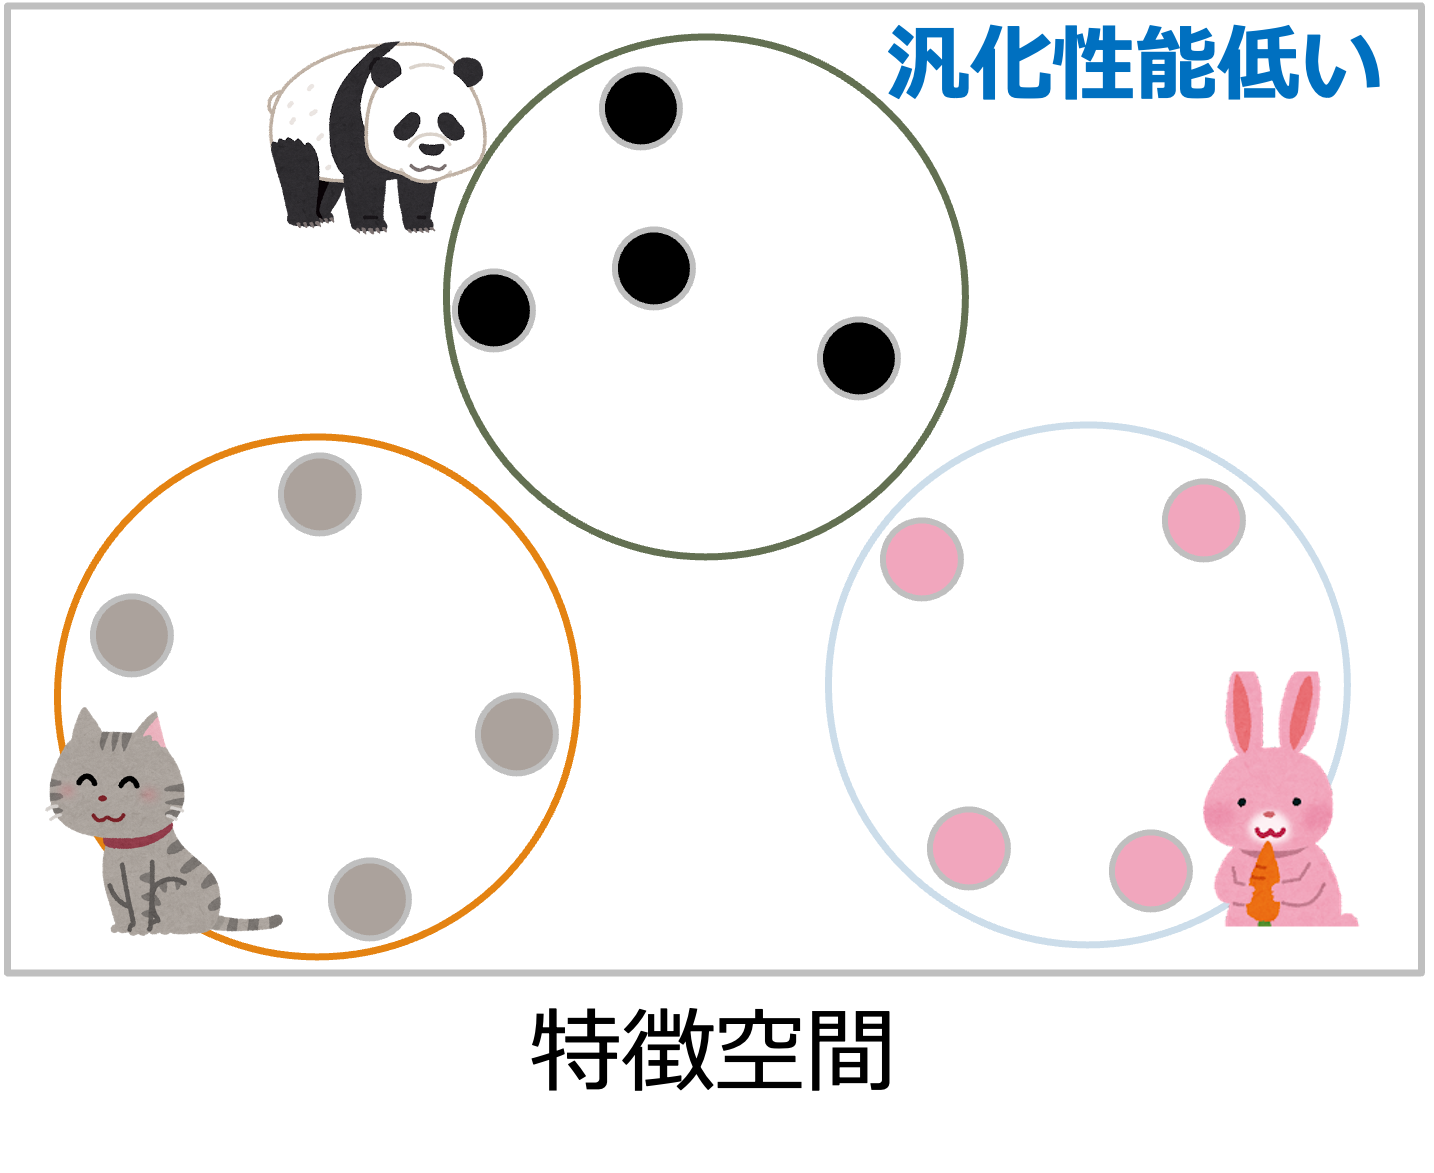
\includegraphics[height=0.9\linewidth, keepaspectratio]{image/bad_featurespace.png}
    \caption{汎化性能の低い特徴空間の例}
    \label{fig:bad_featurespace}
  \end{subfigure}
  \hfill
  \begin{subfigure}[b]{0.45\linewidth}
    \centering
    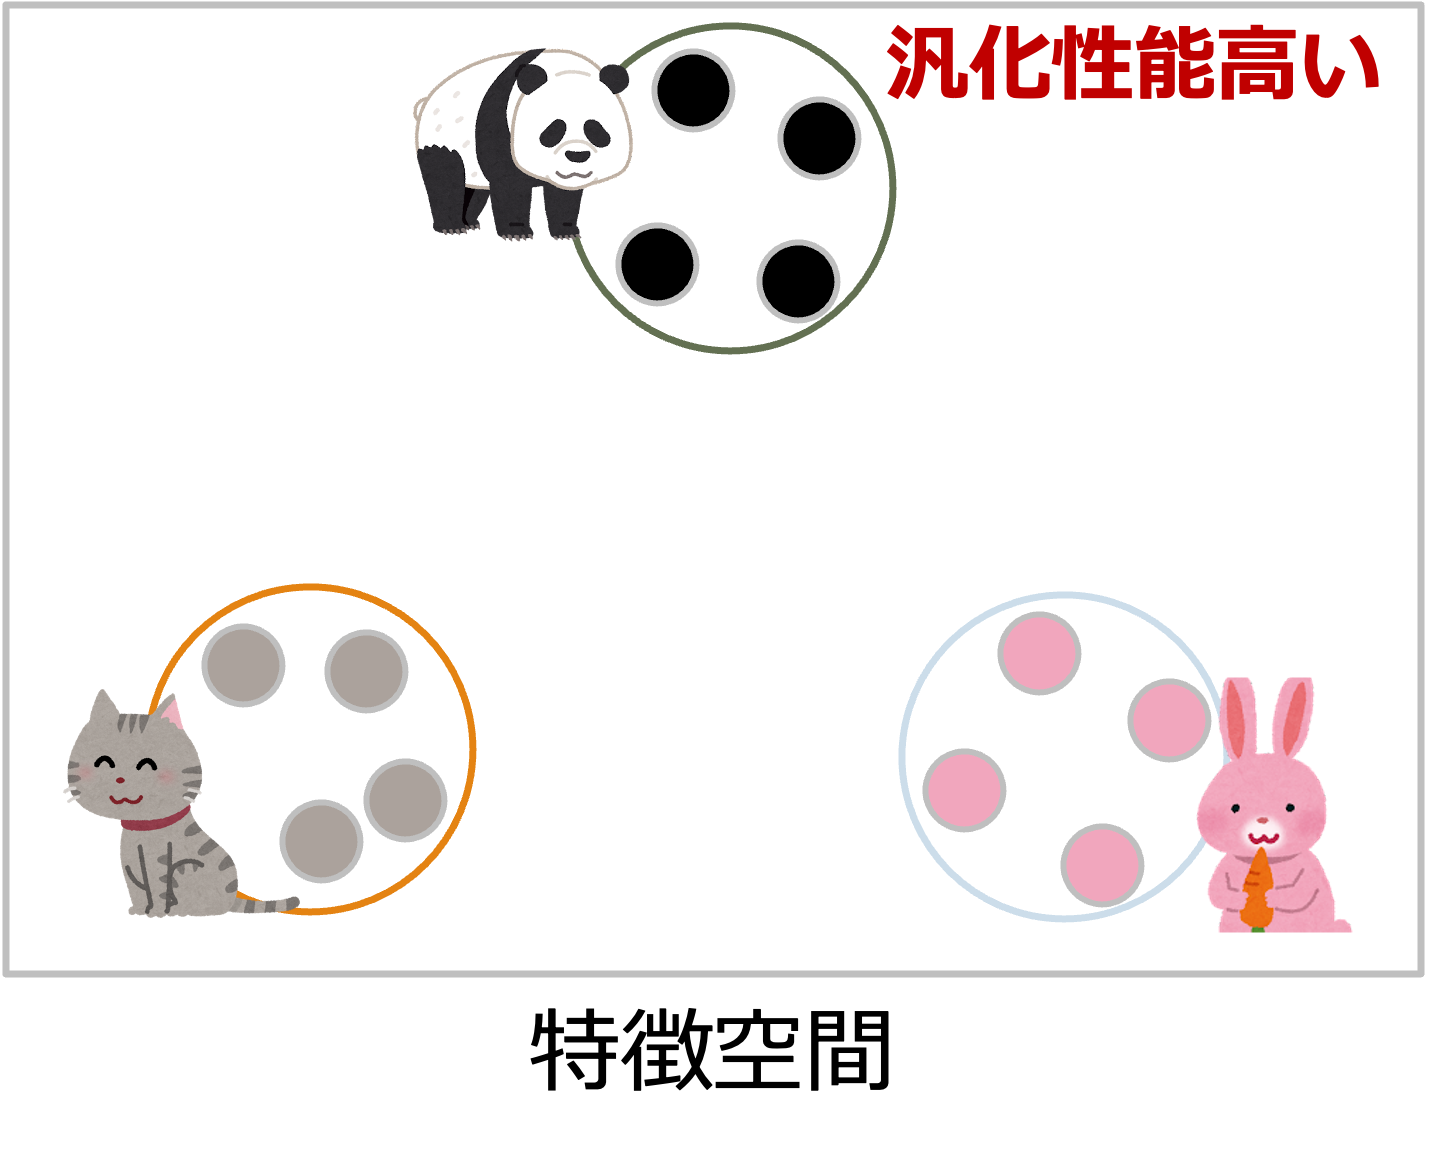
\includegraphics[height=0.9\linewidth, keepaspectratio]{image/good_featurespace.png}
    \caption{汎化性能の高い特徴空間の例}
    \label{fig:good_featurespace}
  \end{subfigure}
  \caption{学習時における特徴空間上の各クラス分布の例}
  \label{fig:feature_space}
\end{figure}
% 
図 \ref{fig:bad_featurespace}および図 \ref{fig:good_featurespace}に示された特徴空間はいずれも同程度の分類精度であるが、ドメインシフトなどを考慮した場合、図 \ref{fig:good_featurespace}の特徴空間の方が、新規地域に対する高い汎化性能を有していると考えられる。
これは、図 \ref{fig:good_featurespace}の方がクラス内分散が小さく、クラス間分散が大きいため、より高い表現力を有しており、新規地域における特徴抽出においても分類が容易となるような特徴空間の構築が期待できるからである。
したがって、本研究では、メタ学習にクラスタリングに基づく損失を導入することによって、クラス内分散の最小化・クラス間分散の最大化を実現し、IFORにおける未登録クラスの多クラス分類精度の向上を目指す。

\subsection{損失関数}

本研究では,FSL損失,OSR損失,分類損失に加え、k-means損失と Between-Class損失 (BC損失) を導入する.
k-means損失は,Chinら \cite{k-means}が異常検知タスクにおいて提案した損失であり,k-meansクラスタリングによって集約される類似した性質を持つ特徴量から,より優れた特徴表現を学習する.
k-means損失による学習の例を図 \ref{fig:kmeans_loss}に示す。
% 
\begin{figure}[tbp]
  \centering
  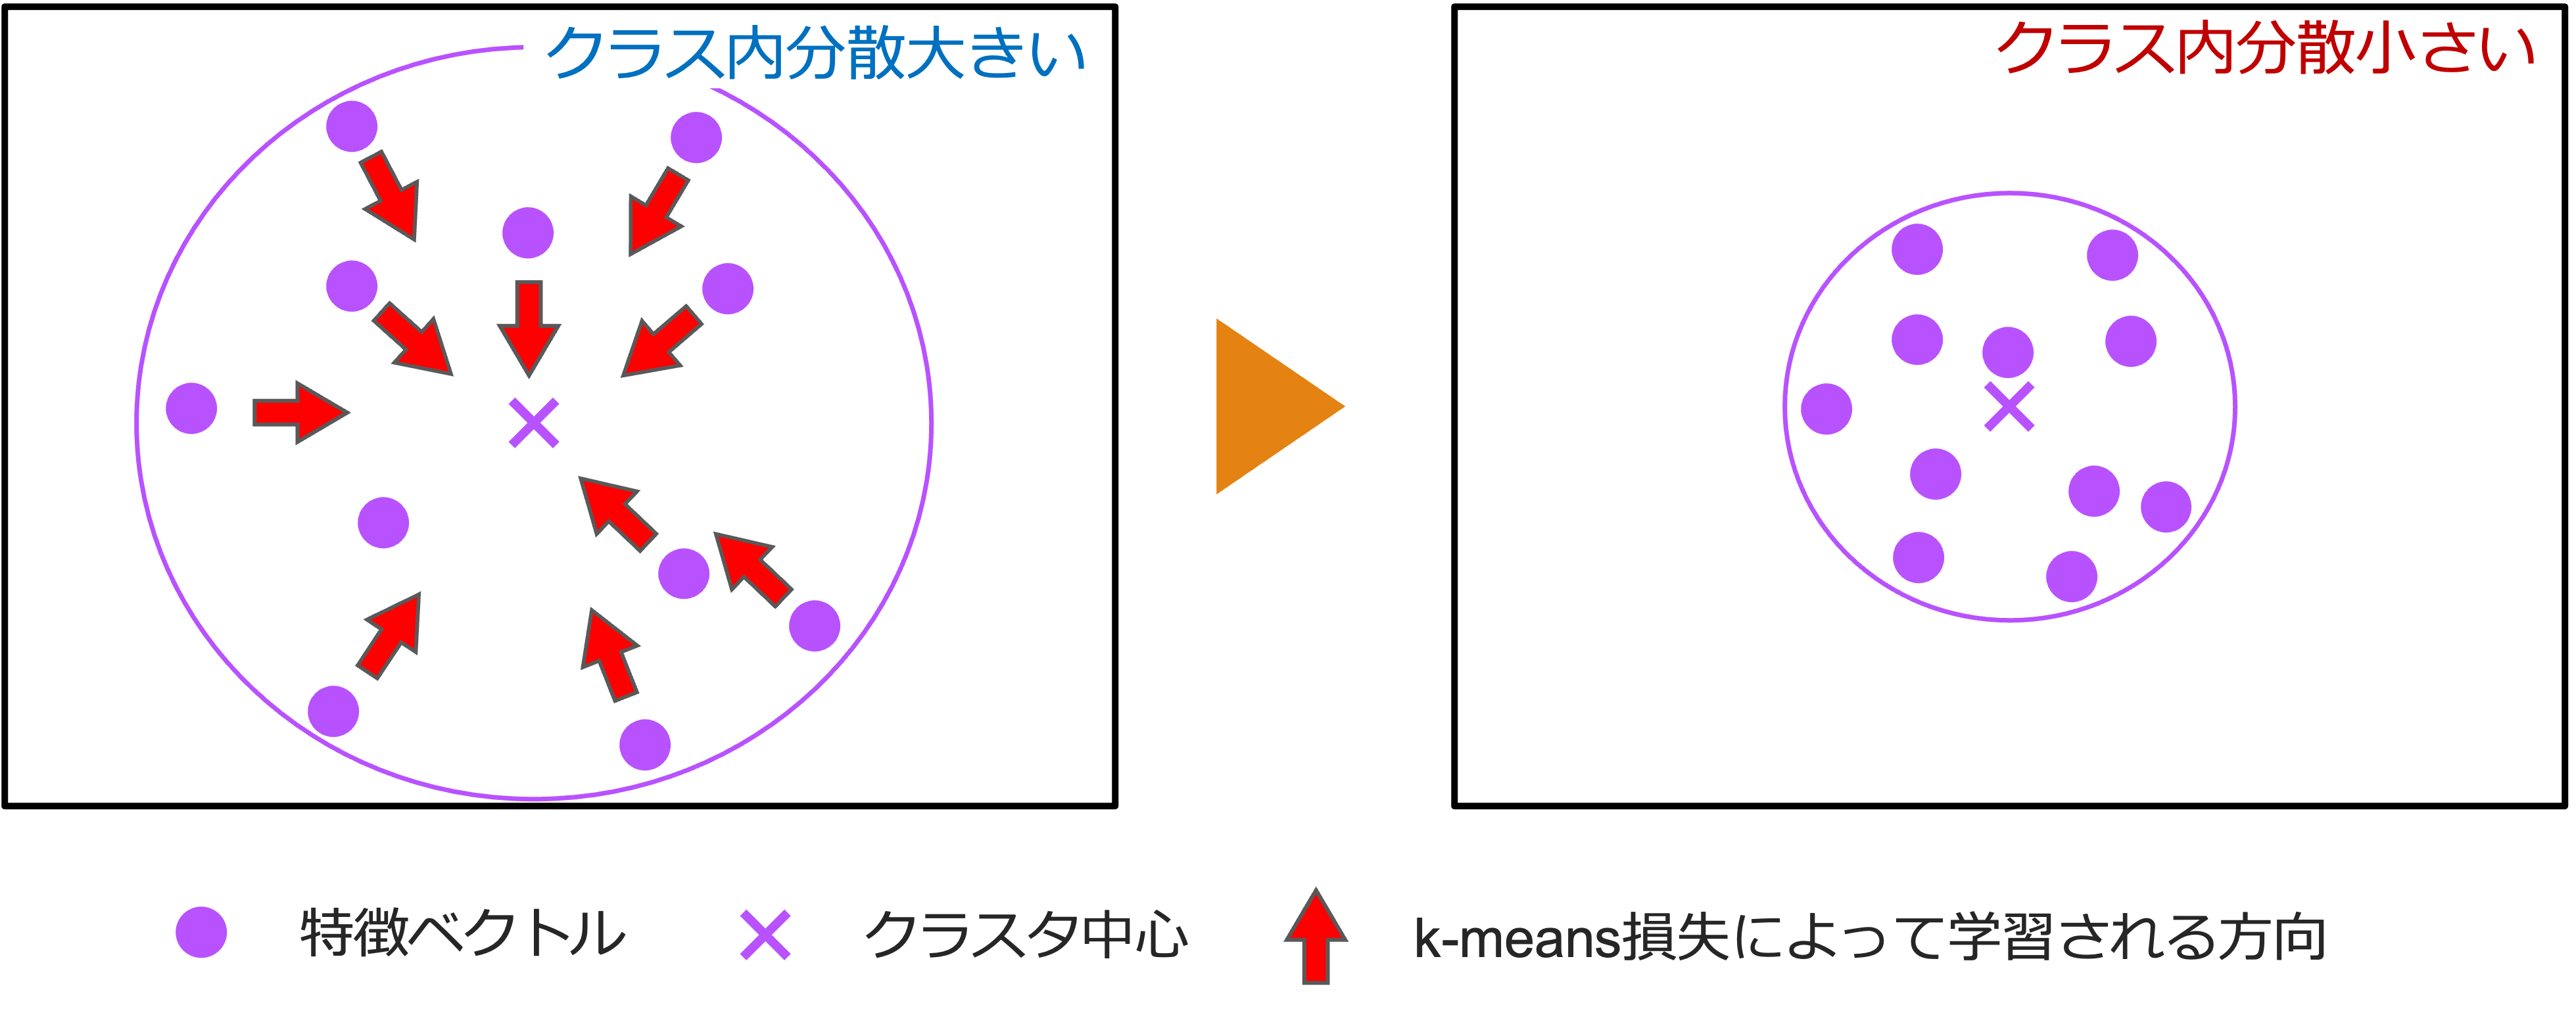
\includegraphics[width=\linewidth, keepaspectratio]{image/kmeans_loss.png}
  \caption{k-means損失によってクラス内分散が小さくなる例}
  \label{fig:kmeans_loss}
\end{figure}
% 
この損失関数では,同一クラスタ内の特徴ベクトルがクラスタ中心に可能な限り近接することが期待される.
本研究では,類似した性質を持つ特徴量のクラスタリングにより,特徴空間上の各クラスのクラス内分散を最小化することを目指し,k-means損失の有効性を検証する.
IFORフレームワークにおいて,k-means損失は以下のように定義される.

\begin{align}
\mathcal{L}_{Kmeans} = \sum_i{\min_k \lVert f(x_i)-c_k \rVert_2}
\end{align}

\noindent
ここで,$f(x_i)$は$i$番目の入力画像を特徴抽出器$f(\cdot)$に入力した際の特徴量,$c_k$は$k$番目のクラスタ中心を表す.

一方,BC損失は,クラス分布のコンパクトな表現に加え、各クラスの分布が可能な限り離れているような特徴空間の構築が、多クラス分類性能の向上に寄与するという考えに基づいている。
BC損失による学習の例を図 \ref{fig:bc_loss}に示す。
% 
\begin{figure}[tbp]
  \centering
  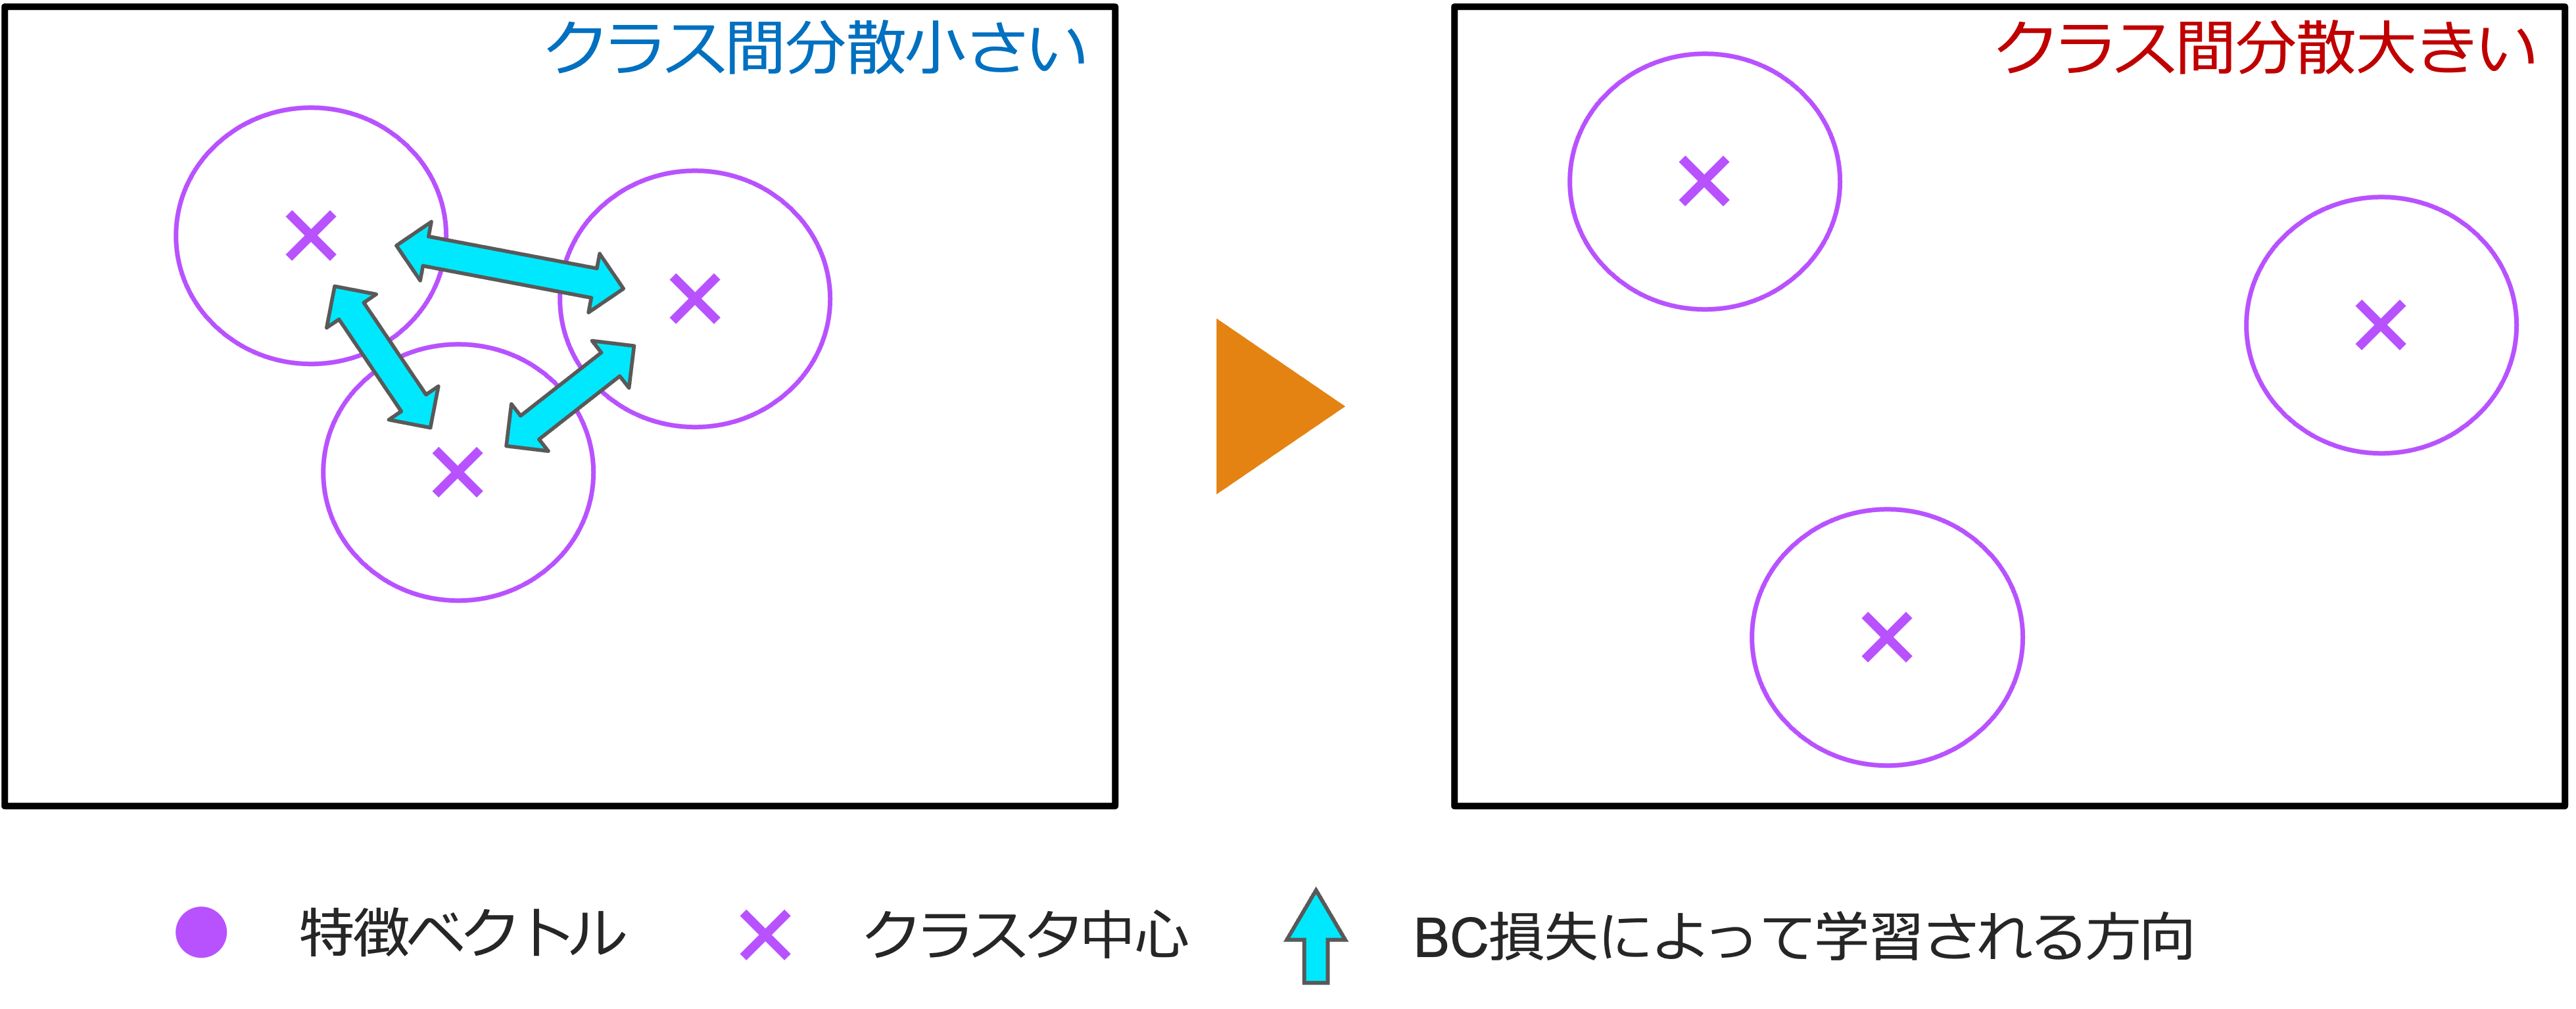
\includegraphics[width=\linewidth, keepaspectratio]{image/bc_loss.png}
  \caption{Between-Class損失によってクラス間分散が大きくなる例}
  \label{fig:bc_loss}
\end{figure}
%
この損失関数では、k-meansクラスタリングによって得られる各クラスタ中心間の距離を最大化することにより,クラス間分散の最大化を目指す。
IFORフレームワークにおいて,BC損失は以下のように定義される.

\begin{align}
  \mathcal{L}_{\text{Between-Class}} = -\log{\sum_{k_1} {\sum_{k_2} {\lVert c_{k_1} - c_{k_2} \rVert_2}}}
\end{align}

\noindent
ここで,$c_{k_1}$と$c_{k_2}$は$k_1$番目,$k_2$番目のクラスタ中心を表す.
負の符号を付与することにより,クラス間分散の最大化問題を損失関数の最小化問題として扱っている.

% ここから参考文献bibtexの設定
\bibliographystyle{../kishiIEEEtr}
\bibliography{../references}

\end{document}